% mn2esample.tex
%
% v2.1 released 22nd May 2002 (G. Hutton)
%
% The mnsample.tex file has been amended to highlight
% the proper use of LaTeX2e code with the class file
% and using natbib cross-referencing. These changes2              
% do not reflect the original paper by A. V. Raveendran.
%
% Previous versions of this sample document were
% compatible with the LaTeX 2.09 style file mn.sty
% v1.2 released 5th September 1994 (M. Reed)
% v1.1 released 18th July 1994
% v1.0 released 28th January 199

\documentclass[useAMS, usenatbib]{mn2e}
%\documentclass[useAMS, usenatbib, doublespacing]{mn2e}
%\documentclass[referee, onecolumn ]{mn2e}
%\pagestyle{empty}
    
% If your system does not have the AMS fonts version 2.0 installed, then
% remove the useAMS option.
%
% useAMS allows you to obtain upright Greek characters.
% e.g. \umu, \upi etc.  See the section on "Upright Greek characters" in
% this guide for further information.
%
% If you are using AMS 2.0 fonts, bold math letters/symbols are available
% at a larger range of sizes for NFSS release 1 and 2 (using \boldmath or
% preferably \bmath).
%
% The usenat  command allows the use of Patrick Daly's natbib.sty for
% cross-referencing.
%
% If you wish to typeset the paper In Times font (if you do not have the
% PostScript Type 1 Computer Modern fonts you will need to do this to get
% smoother fonts in a PDF file) then uncomment the next line
% \usepackage{Times}

%%%%% AUTHORS - PLACE YOUR OWN MACROS HERE %%%%%


\usepackage{graphicx}
\usepackage{aas_macros}
\usepackage{amsmath, amssymb}
\usepackage{array}
\usepackage[usenames,dvipsnames]{color}
\usepackage{multirow}
\usepackage{threeparttable}
\usepackage{comment}
\usepackage{float}



\newcommand{\vdag}{(v)^\dagger}
\newcommand{\myemail}{Mohammad.Nawaz@anu.edu.au}

\newcommand{\noteM}[1]{\textbf{\textcolor{NavyBlue}{$^\mathrm{Mohammad}$ #1}}}
\newcommand{\noteA}[1]{\textbf{\textcolor{SeaGreen}{$^\mathrm{Alex}$#1}}}
\newcommand{\noteG}[1]{\textbf{\textcolor{RedOrange}{$^\mathrm{Geoff}$#1}}}


\title[Jet-ICM interaction of Hydra A]{Jet-Intracluster Medium interaction in Hydra A. II The Effect of Jet Precession}
\author[M. A. Nawaz et al.]{
M.~A. Nawaz$^{1}$,\thanks{E-mail Mohammad.Nawaz@anu.edu.au} 
G.~V. Bicknell$^{1}$,
A.~Y. Wagner$^{2}$,
R.~S. Sutherland$^{1}$ 
and B.~R. McNamara$^{3}$
\\
$^{1}$ Research School of Astronomy and Astrophysics, The Australian National University, ACT 2611, Australia; \myemail \\
$^{2}$ Center for Computational Science, Tsukuba University, 1-1-1 Tennodai, Tsukuba, Ibaraki, 305-8577 Japan \\
$^{3}$ Department of Physics and Astronomy, University of Waterloo, Waterloo, ON N2L 2Y5, Canada}

\begin{document}


\date{Accepted 2013 July ??. Received 2013 July ??; in original form 2013 July ??}

\pagerange{\pageref{firstpage}--\pageref{lastpage}} \pubyear{2013}

\maketitle

\label{firstpage}

\begin{abstract}
\noteA{Modified first two sentences of the abstract - please check.}
We present three dimensional relativistic hydrodynamical simulations of a precessing jet interacting with the intracluster medium and compare the simulated jet structure with the observed structure of the Hydra A northern jet. For the simulations, we use jet parameters obtained in the parameter space study of Paper I, and probe different values for the precession period and precession angle. We find that for a precession period $\approx 1 \> \rm Myr$ and a precession angle $\approx 20^{\circ}$ the model reproduces i) the curvature of the jet, ii) the correct number of bright knots within 20~kpc at approximately correct locations, and iii) the turbulent transition of the jet to a plume. We also present a possible explanation for a misaligned knot at approximately 12~kpc from the core. The Mach number of the advancing bow shock $\approx 1.85$ is indicative of gentle cluster atmosphere heating during the early stages of the AGN's activity. Assuming that the jet precession is associated with the AGN accretion disk, we estimate the viscosity parameter of the accretion disk $0.03\le \alpha \le 0.15$. 
\end{abstract}

%% GVB: Are the bright knots at the correct location?

\begin{keywords}
TBD
\end{keywords}


%%%%%%%%%%%%%%%%%%%%%%%%%%%%%%%%%%%%%%%%%%%%%%%%%%%%%%%%%%%%%%%%%%%%%%%%
%
%												Introduction
%
%%%%%%%%%%%%%%%%%%%%%%%%%%%%%%%%%%%%%%%%%%%%%%%%%%%%%%%%%%%%%%%%%%%%%%%%
\section{Introduction}
%GVB
Morphologically, extragalactic radio sources have either straight jets or have complex curved morphologies with C or S shaped\footnote{this is sometimes referred to as X or Z symmetry} symmetry \citep{zaninetti88}. In general, C-symmetric jets are explained by the motion of the host galaxy with respect to the intergalactic medium \citep{morsony13}.
However, for S-symmetry there are three possible explanations: -- jet deflection by buoyancy \citep{kraft05}, jet deflection of back flows \citep{hodges-kluck11} and jet precession \citep{kurosawa08}.

In many cases, for an S-symmetric structure jet precession is an attractive interpretation. The idea of jet precession was first introduced by \citet{ekers78} who interpreted the S-shaped structure of the radio morphology of NGC326 as a result of the precessional motion of the jets. Subsequently, utilising an analytical model, \citet{gower82} showed that the curved jet morphologies of a number of radio galaxies may be attributed to jet precession.

\noteA{New paragraphs below, some sentences borrowed from Brian's email comments. Please check. Citations still needed.}
It is now generally accepted that AGN jets in massive cluster galaxies are responsible for inhibiting cooling flows in the hot intracluster medium (ICM) and shaping the bright end of the galaxy luminosity function \citep{croton2006a, fabian2012a, mcnamara2012a}. The AGN jets of radio galaxies certainly have sufficient kinetic power to heat the ICM and counteract radiative cooling, and occur in the majority of cluster central galaxies, in particular if they exhibit a cool core \citep{mittal2009a}  . However, the details of the energy transfer from relativistic jet plasma to the internal energy of the gas are not well understood. Some combination of shock heating, entrainment, thermal conduction, and magnetohydrodynamic turbulence is involved \citep{}, but the relative importance of these is not known. As a result, this form of feedback, often termed ``radio-mode'' feedback, is often incorporated in rudimentary ways in cosmological simulations, e.g. by injecting a spherical region with internal energy or stopping cooling in the halos of galaxies for some duration of the simulation \citep{}. It is, therefore, very important to conduct thorough (magneto-)hydrodynamical modelling of well-observed sources exhibiting radio-mode feedback such as Hydra A, in order to pin down the heating mechanisms in AGN feedback.

Even basic assumptions of jet-ISM interactions are problematic. \cite{vernaleo2006a} highlighted, using 3-dimensional hydrodynamical models, that strait jets advancing into static atmospheres will punch through the gas, with much of the mechanical energy escaping to large radii. They found that cooling flows were inevitable because insufficient solid angle was in the case of feedback straight jets, and they pointed out that the ``dentist drill effect'', i.e. precession, and atmospheric motions driven by normal merging would enhance the coupling between the jet and ambient gas. For example, \citet{heinz2006a} showed with hydrodynamic simulations that bulk intracluster gas motions allow the jet to impact a larger volume of gas including cooled gas that would be out of the jet's reach in a static cluster atmosphere, and allow for a stronger interaction by collapsing the channels formed by the jets. 

Several attempts have been made to model the interaction between a precessing jet and the ambient medium numerically. Using three dimensional numerical simulations, \citet{cox91} showed that multiple hotspots of jets in radio sources are produced when the jets change their direction as a result of precessional motion. \citet{hardee01} computed 3D models of a precessing cylindrical jet and discussed the jet knots as a result of the wave-wave interactions of the body mode and surface mode of the Kelvin-Helmholtz (KH) instability. They applied their model to the inner knots of M87. \citet{kurosawa08} modelled a precessing jet originating from a precessing accretion disk with a range of precession periods and precession angles. They showed that jet precession is able to produce S- or Z-shaxped structures. In this paper, we show that the internal 20~kpc structure of Hydra A jet can also be modelled by a precessing jet and based on a parameter space study we estimate the precession period and precession angle.
 
The radio galaxy Hydra A, located at the centre of the galaxy cluster Abell 780, shows a spectacular S-shaped morphology within the central 20~kpc. The symmetrical S-structure is also visible in the extended low frequency images at 74 and 330~MHz \citep{lane04}; the radio source is extended by approximately 340~kpc in the north and by 190~kpc in the south. Modelling the entire source is computationally impractical and we have adopted the approach of modelling the innermost structures first in order to constrain jet parameters \citep[][hereafter Paper I]{nawaz14a}, then utilising these parameters model the intermediate scale structure (this paper) and finally the large scale structure. 

In Paper I we commenced our study of Hydra A focussing on the central 10~kpc structure of the northern jet. We studied the kinetic power of the Hydra A jets and two key features of the inner 10~kpc of the northern jet: i) the oscillatory jet boundary and ii) two bright knots at approximately 3.7~kpc and 7.0~kpc. Since the jet is mildly bent within 10~kpc, we used two dimensional axisymmetric simulations and modelled the inner two bright knots as biconical reconfinement shocks. By fitting the knot location and the radius profile of the observed jet with our models we estimated the jet velocity at 0.5~kpc to be approximately 0.8c, the jet over pressure ratio  with respect to the ICM to be approximately 5, and the jet density parameter to be approximately 13. 

In the present study we address the following additional key features of the inner 20~kpc of the northern Hydra A jet: i) the curved jet morphology, ii) two additional bright knots beyond 10 kpc and iii) the turbulent transition of the jet to a dissipative plume. In Fig.~\ref{f:obs} we show the radio structure of the northern jet and indicate these features. This figure is produced using the 4.635~GHz VLA data (G. Taylor, priv. comm.). The detailed description of these data is available in \citet{taylor90}. In order to model the curved jet morphology we use a three dimensional relativistic hydrodynamical model of a precessing jet based on the jet and interstellar medium (ISM) parameters obtained in Paper I. 

In outline, our model for the Hydra A northern jet is as follows: The initially conical, precessing jet expands through the ambient medium. The curvature of the jet is caused by its precessional motion.
As a result of the interaction between the jet and the ISM a series of biconical reconfinement shocks which manifest themselves as bright knots appear along the jet axis as in our straight jet models in Paper I. The collimated jet starts to become turbulent when it is sufficiently decelerated by the recollimation shocks. The turbulent jet hits the dense cocoon wall near the fourth knot and the backflowing jet plasma creates a strong turbulent dissipative zone (marked by a shadowed ellipse in Fig.~\ref{f:obs}).
 

The paper is structured as follows. In Section~\ref{s:model} we present a detailed description of our model of the precessing jet-ISM interaction. The results of the numerical models are presented in Section~\ref{s:results}. We summarise and discuss our results in Section~\ref{s:discussion}. 


%%%%%%%%%%%%%%%%%%%%%%%%%%%%%%%%%%%%%%%%%%%%%%%%%%%%%%%%%%%%%%%%%%%%%%%%
%
%												Details of the model
%
%%%%%%%%%%%%%%%%%%%%%%%%%%%%%%%%%%%%%%%%%%%%%%%%%%%%%%%%%%%%%%%%%%%%%%%%
\section{Details of the model}\label{s:model}
\begin{figure}
\centering
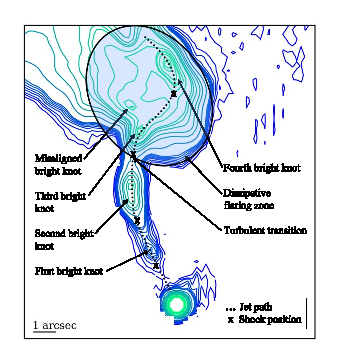
\includegraphics[width=\linewidth]{fig1.eps}
\caption{Radio intensity map of the central 20~kpc of the Hydra A northern jet at 4.635 GHz. Contour levels are at 1.5, 2.7, 3.7, 5.1, 6.3, 7.5, 8.8, 10, 21, 37, 51, 72, 90, 103, 150, 180, 200, 205, 220, 240 and 249 mJy arcsec$^{-2}$. Four bright knots are marked with black arrows. The locations of the biconical reconfinement shocks which we interpret as the cause of the bright knots \citep{nawaz14a} are marked with $\times$. An imaginary jet path is traced by a dotted line following the ridge line and joining the four knots. Near the third knot there is a bright knot, marked as 'misaligned knot', which is not aligned with the jet trajectory. The turbulent transition of the jet starts at the location marked by an arrow. The elliptical shaded area outline a dissipative zone.}
\label{f:obs}
\end{figure}

The motivation for this study is to understand the dynamical interaction of the inner Hydra A northern jet with the interstellar medium and cluster environment and to understand the reason for the source morphology. Therefore, we mainly focus on the features of the inner 20~kpc including i) the curved jet ii) the four bright knots at approximately 3.7~kpc, 7.0~kpc, 11.0~kpc and 16.0~kpc from the core (deprojected) iii) the turbulent transition of the jet to plume at approximately 10~kpc from the core, and iv) the bright radio emission region at approximately 10 to 20~kpc from the core. 

In Paper I, using axisymmetric straight jet simulations we modelled the first two bright knots of the northern jet as biconical reconfinement shocks. Here we develop this model by introducing precession of the jet and this necessitates three dimensional simulations.  According to our model, the jet is initially ballistic and conically expands in the first 0.5~kpc. It then starts to interact with the ISM and is collimated by the ambient pressure. A series of bright knots are produced along the jet path at the locations of the biconical reconfinemnet shocks. 

The initially supersonic jet is decelerated significantly by the first two reconfinement shocks and the jet starts to form a turbulent plume at approximately 11~kpc from the core. The jet strongly interacts with the ISM and produce further reconfinement shocks at approximately 11~kpc and 16~kpc. Some jet plasma is deflected by the dense cocoon wall near the fourth knot and a highly turbulent zone is established in the region of approximately 11-20~kpc. 

Note that in the northern Hydra A jet there is a bright knot (marked by 'mis-aligned knot') that is not aligned with the jet path (the black dotted line in Fig.~\ref{f:obs} inferred by following the ridge line and connecting the four bright knots). Prior to conducting our simulations there was no indication as to how this misaligned knot actually formed. 

Our modelling strategy is as follows. We conduct a small parameter space study with jet parameters derived from the best fit axisymmetric model of Paper I, a range of precession periods and two values of the precession angle. We then construct synthetic surface brightness images of the models and compare the source morphology obtained from our models with the observations. Matching the key features, namely, the curvature of the jet, the locations of the bright knots and the turbulent transition of the jet to a plume, we select a best model. 

%%%%%%%%%%%%%%%%%%%%%%%%%%%%%%%%%%%%%%%%%%%%%%%%%%%%%
%
%						Numerical Setup
%
%%%%%%%%%%%%%%%%%%%%%%%%%%%%%%%%%%%%%%%%%%%%%%%%%%%%%
\subsection{Precession geometry, simulation setup and parameters}
\begin{figure}
\centering
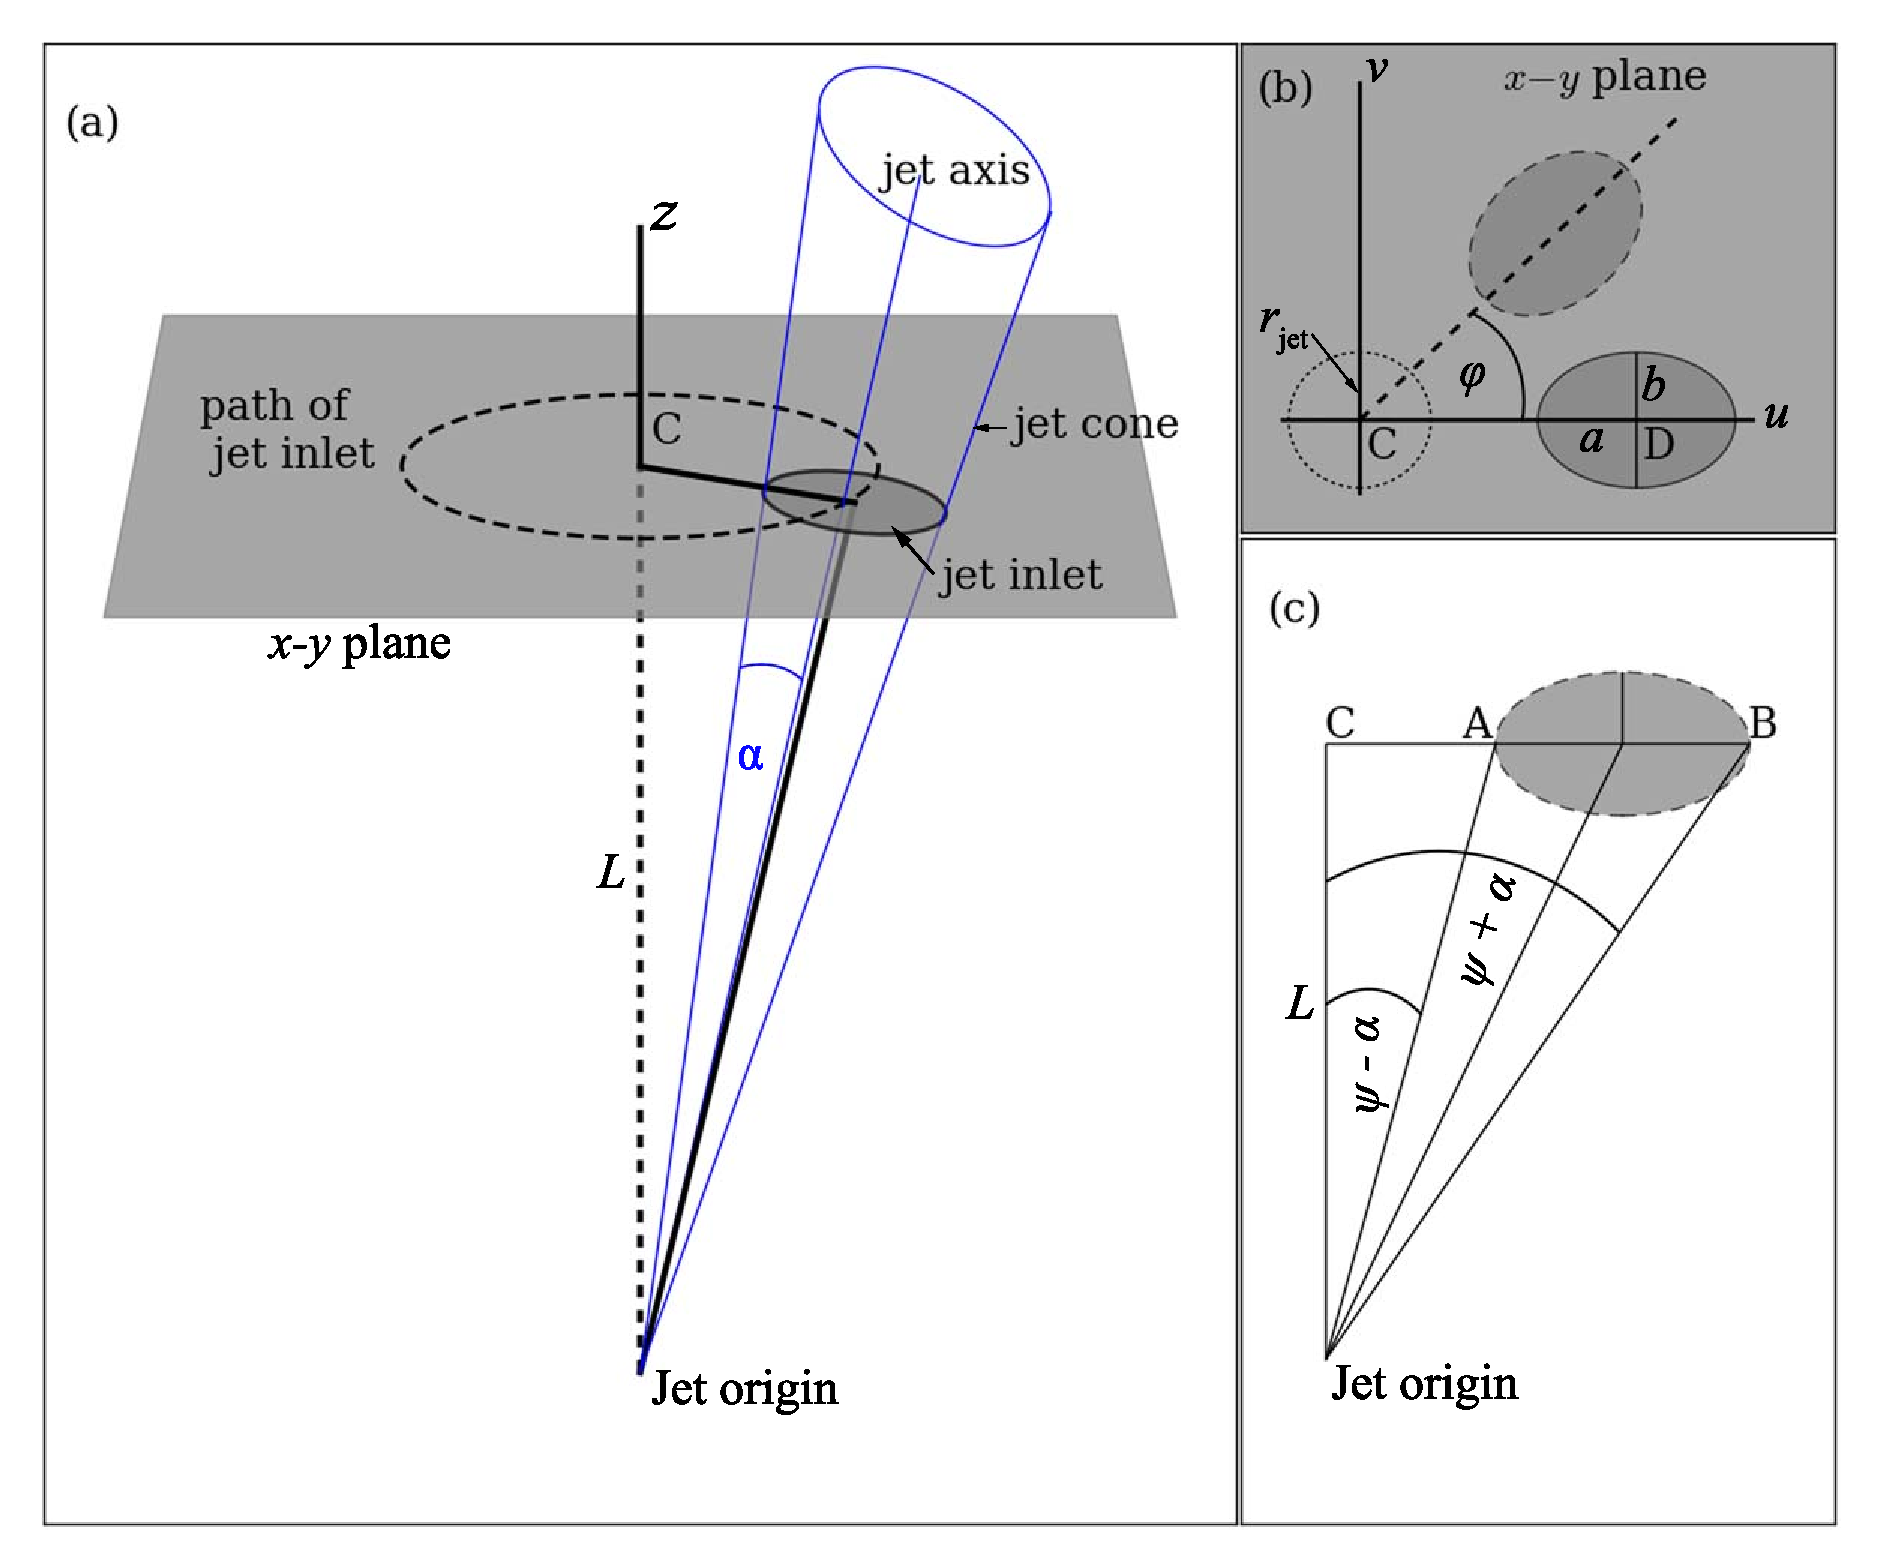
\includegraphics[width=\linewidth]{fig2.eps}
\caption{Geometry of the precessing jet model. Panel (a) shows  the conical jet originating at a distance $L$ below the $x-y$~plane of the computational domain. The precessing jet cone intersects the $x-y$~plane in an elliptical jet inlet which moves on the (dashed) circular path. The coordinates $(u,v)$, defined by the intersection of the cone and the $x-y$~plane at a precession azimuth $\phi = 0^{\circ}$ and an arbitrary $\phi$ are shown in panel (b). The dotted circular line is the intersection of the cone when the precession angle $\psi = 0^{\circ}$.
The jet semi-minor axis of the jet inlet $b$ is equal to the jet radius $r_{\rm jet}$.  In panel (c) the angles defined by the lines joining the jet origin and the left and right edges of the inlet ellipse are shown. These define the semi-major axis of the ellipse.}
\label{f:mod}
\end{figure}
The geometrical configuration of our precessing jet model for the Hydra A northern jet is shown in Fig.~\ref{f:mod}.  The jet originates near the central black hole (marked as the jet origin in panel (a)) and is initially ballistic and conically expanding \citep{komissarov98, krause12, nawaz14a}. It precesses around the $z$-axis with a precession period $P$ and a precession angle $\psi$. The best fit axisymmetric model (presented in Paper I) gives a jet radius $r_{\rm jet} = 0.1$~kpc at $L=0.5$~kpc away from the black hole. The half cone angle of the jet cone is then $\alpha = \tan^{-1}(r_{\rm jet}/L) = 11.3^{\circ}$.

The jet cone intersects the $xy$~plane at a distance $L$ from the central black hole in an ellipse. As a result of precession the elliptical jet inlet follows a circular path (marked in panel (a)) on the $xy$~plane. The elliptical jet base is determined from the geometry shown in panels (b) and (c) of Fig.~\ref{f:mod} as described below.  

Let $(u,v)$ be a rotating frame fixed on the elliptical jet inlet. The semi-major axis $a$ and semi-minor axis $b$ of the ellipse lie on the $u$ and $v$ axes respectively (see panel (b) of Fig.~\ref{f:mod}). The centre of the ellipse lies at 
\begin{eqnarray}
u_0 = L[\tan(\psi+\alpha) - \tan(\psi - \alpha)]/2, \\
v_0 = 0.
\end{eqnarray}
%GVB
%From the geometry of panel (b) and (c) we obtain 
From the geometry described in panels (b) and (c) we obtain 
\begin{eqnarray}
a &=& L[\tan(\psi + \alpha) - \tan(\psi -\alpha)]/2, \\
b &=& r_{\rm jet}.
\end{eqnarray}
Therefore, in the rotating $(u,v)$ coordinate system the jet inlet is defined by 
\begin{equation}
(u - u_0^2)/a^2 + v^2/ b^2 \leq 1.
\end{equation}
%GVB
% State why you want to use this coordinate transformation; Also presumably \theta should be \phi? Also, \phi should be defined in Fig. 2.
%For a counter-clockwise rotation of the jet inlet the body fixed coordinates $uv$ are obtained from the computation coordinates $xy$: 
For a counter-clockwise rotation of the jet inlet the coordinates $uv$ are related to the computational coordinates $xy$: 

\begin{eqnarray}
u &=& x\cos \phi + y \sin \phi, \\
v &= &- x \sin \phi + y \cos \phi,
\end{eqnarray} 
%aln
here $\phi = 2\pi t/P$ is the azimuth angle of the precession. 


In order to avoid reverse shocks running through ghost zones we initialise the jet in the computational domain with a semi-ellipsoidal cap above the jet inlet with semi-principle axes $a, \ b$ and $c (= a)$. 


The input jet parameters, the jet kinetic power $P_{\rm jet} = 1\times 10^{45}$~erg s$^{-1}$, the jet over-pressure ratio $p_{\rm jet}/p_{\rm a} = 5$, the jet velocity $\beta = 0.8$, and the jet density parameter $\chi = 12.75$ are chosen from the best fit axisymmetric model presented in Paper I. We explore a range of values for the precession period $P = 1, 5, 10, 15, 20, 25$~Myr and the precession angle $\theta = 15^{\circ} \rm \ and \ 20^{\circ}$. The grid of models is presented in Table~\ref{t:mod}. Since the radiative cooling time of the environment is large compared to the simulation time, we do not include cooling in our models. 

As described in Paper I, the three-dimensional cluster environment is constructed using analytical fits for the density, pressure and temperature data derived from the X-ray data presented by \citet{david01}.
 
We set up the computational grid as follows. We use a high resolution $156^3$ uniform grid for the inner 5~kpc$^3$, thereby resolving the jet base by six cells. For the remaining computational domain we use stretched grid with 100 additional cells along each of the coordinate directions. 

The simulations were performed with the publicly available relativistic hydrodynamic code PLUTO \citep{mignone07}, which solves the relativistic gas dynamical equations using the finite volume method based on Godunov type schemes. 

\begin{table*}
\centering
\caption{Grid of precessing jet-ICM interaction model. }
\begin{threeparttable}
\begin{tabular}{*{7}{c}}
\hline \hline
%GVB
% Models &   $P$ & $\theta$  & Computation domain  \\
Model &   Period & Precession   \\
      & (Myr)  & angle (degrees) \\ 
 \\ \hline
   A & 1.0 & 20 \\
   B & 1.0 & 15  \\
   C & 5.0  & 20  \\
   D & 10.0 & 20 \\
   E & 15.0 & 20 \\
   F & 20.0 & 20 \\
   G & 25.0 & 20 \\
\hline
\end{tabular}
\label{t:mod}
\end{threeparttable}
\end{table*}

%%%%%%%%%%%%%%%%%%%%%%%%%%%%%
%
%			Synthetic surface brightness
%
%%%%%%%%%%%%%%%%%%%%%%%%%%%%%
\subsection{Synthetic surface brightness}
\begin{figure*}
\centering
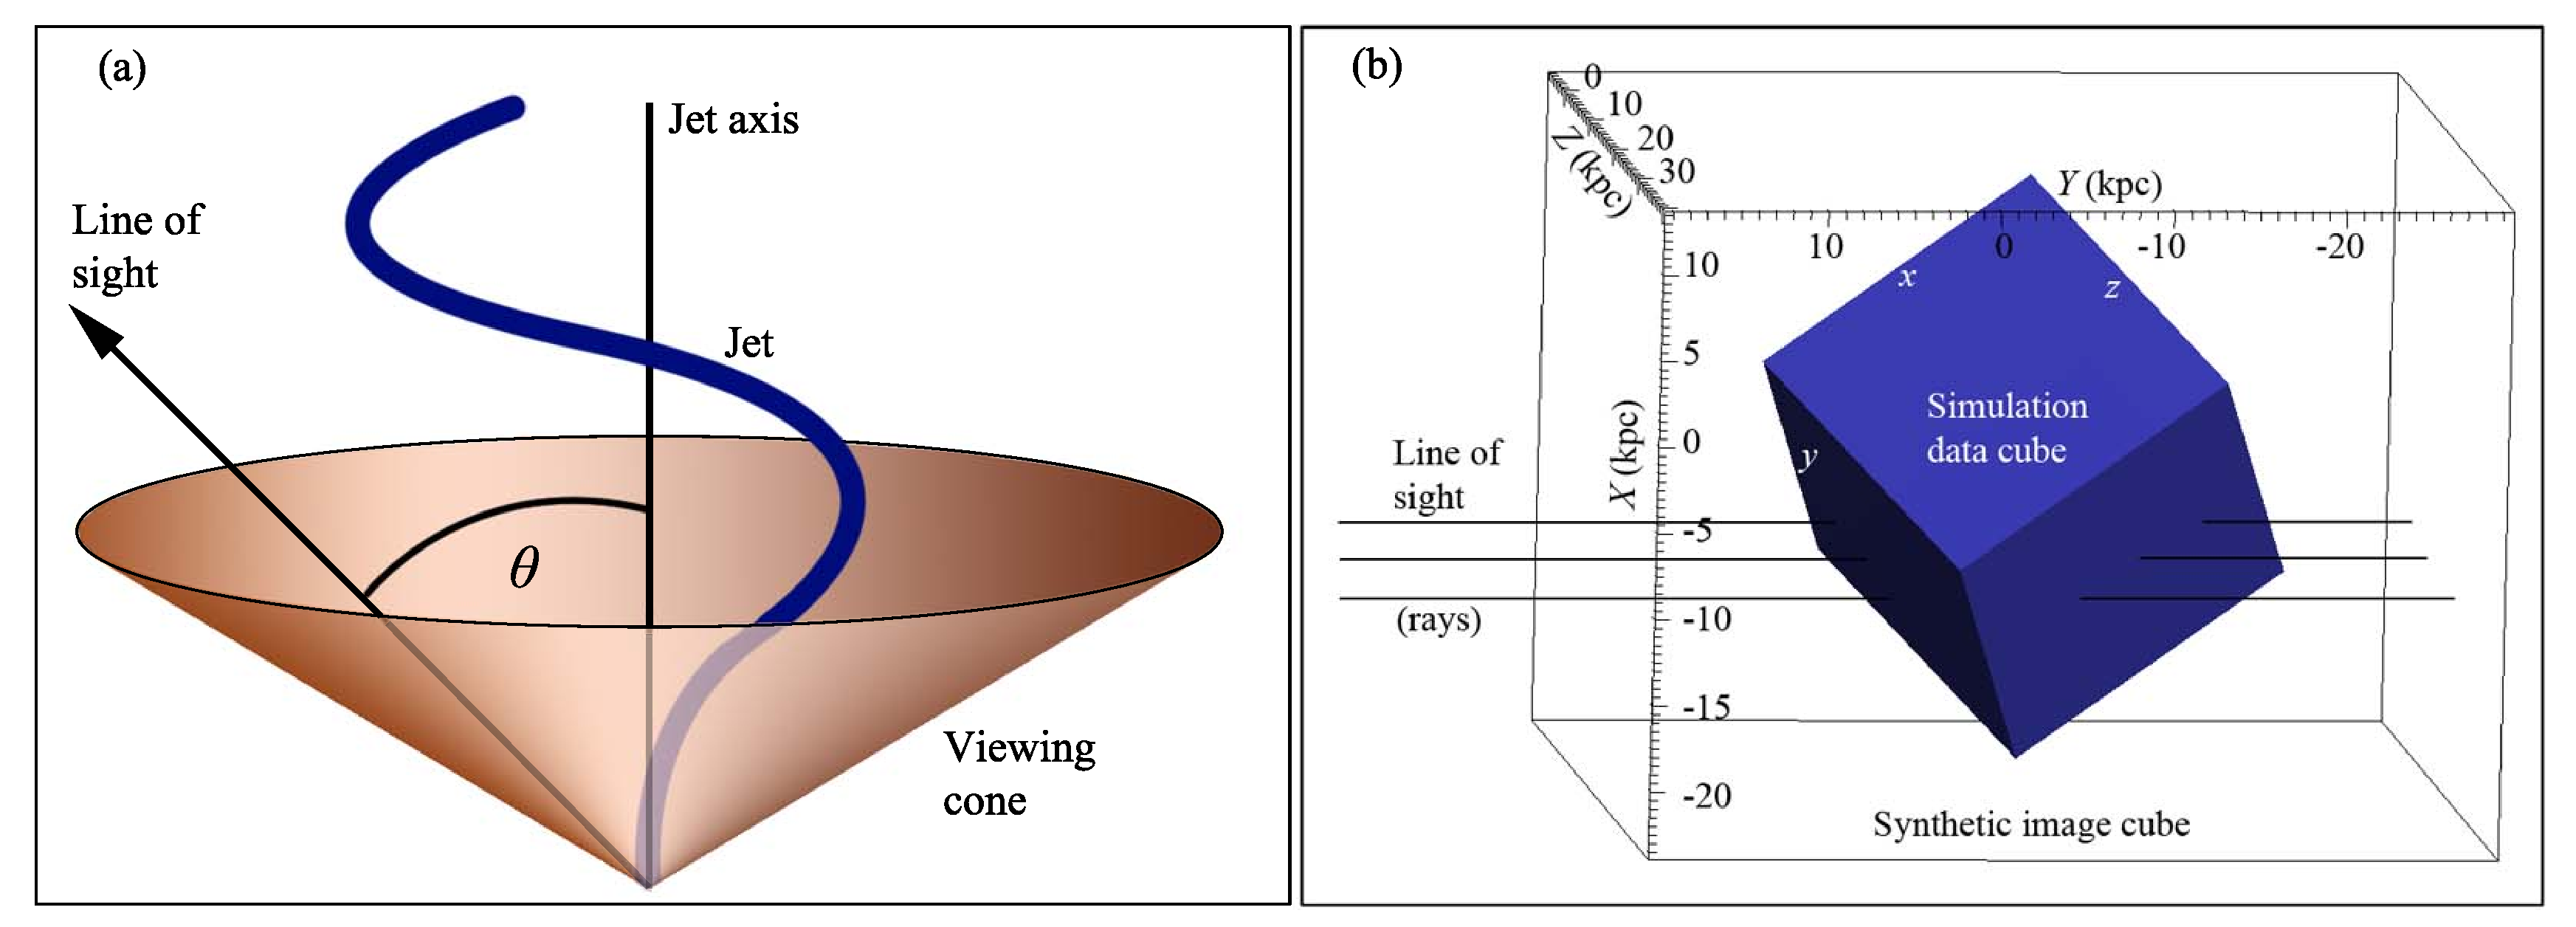
\includegraphics[width=\textwidth]{fig3.eps}
\caption{Dependencies of the jet morphology on the line of sight and the viewing direction. (a) A cartoon of a spiral jet, an arbitrary line of sight and a viewing cone with cone axis aligned with the jet axis and cone angle equal to the line of sight angle are shown. Any line of sight lying on the viewing cone has the same inclination $\theta$ with the jet axis. The observed source morphology depends on both the line of sight inclination $\theta$ and the viewing direction. (b) The image cube, the data cube and the line of sight (marked by rays) are shown. The data cube is rotated with respect to the image cube to obtain any line of sight and a viewing direction.}
\label{f:con}
\end{figure*}

In order to compare the morphologies derived from the models with the radio observations we produce synthetic surface brightness images for each model. Following \citet{sutherland07}, we use a synchrotron rest-frame emissivity $j_\nu \propto p^{(3+\alpha)/2}$ where  $\alpha$ is the spectral index.  In this expression, the magnetic pressure is assumed to be proportional to the non-thermal particle pressure. The northern Hydra A jet is approaching towards the observer and hence the emissivity $j_\nu$ is modified by the Doppler factor $\delta = 1/\Gamma(1 - \beta \cos\theta]$, where $\Gamma$ is the bulk Lorentz factor and $\theta$ is the angle between the jet axis and the line of sight. In addition, to isolate the jet plasma from the ambient medium we use a tracer $\lambda$, which is the mass concentration of plasma at each cell. We initialise the jet plasma with a value $\lambda = 1$. Hence the emissivity $j_\nu$ becomes 
\begin{equation}
j_\nu = \lambda \delta^{2+\alpha}p^{(3+\alpha)/2}
\end{equation}
Integrating the synchrotron emissivity along rays, parallel to the line of sight, $I_\nu = \int j_\nu ds$, we obtain images of the synthetic surface brightness of the modelled jets. 

We note that the source morphology depends on both the angle between the jet axis and the line of sight and the viewing direction in azimuth. For instance, Fig.~\ref{f:con} shows an arbitrary spiral jet structure about the jet axis and an arbitrary line of sight (making an angle $\theta$ with the jet axis). In this figure a viewing cone is also shown. The axis of the viewing cone lies along the jet axis and its cone angle is equal to the inclination of the line of sight $\theta$. Any line of sight lying on the viewing cone has the same inclination $\theta$ but different azimuthal direction. It is clear from this figure that the jet morphology is different if either $\theta$ or the azimuth direction or both change. Therefore, we scan the synthetic images for different lines of sight and azimuth until we obtain the best match of the synthetic surface brightness to the observations. 

In using the VisIt visualisation software\footnote{https://wci.llnl.gov/simulation/computer-codes/visit/}, it proved to be expedient to work with a fixed image cube and to rotate the computed emissivity cube with respect to this image cube in order to investigate the dependence of the synthetic image on viewing direction. The data cube is rotated so that the line of sight along which the surface brightness is calculated is the $Y$-axis of the image cube. We perform four successive rotations of the data cube ($xyz$) with respect to the image cube ($XYZ$) to obtain a desired line of sight and viewing direction. Details of the transformations are presented in the Appendix~\ref{A:trans}. 

Let $\textbf{v}'$ and $\textbf{v}$ be the velocity vector of the fluid in the image cube and data cube respectively. Then the velocity $\textbf{v}'$ is given by 

\begin{equation}
\textbf{v}' = R \textbf{v}
\end{equation}
where R is the transformation matrix (see Appendix~\ref{A:trans} for the description of $R$).

The angle between the line-of-sight ($Y$-axis) and the fluid velocity at a cell is given by 
\begin{equation}
\theta' = \cos^{-1}v'_Y / v'
\end{equation}
where $v'_Y$ and $v'$ are the $Y$ component and magnitude of the velocity in the image cube, respectively. To obtain the correct Doppler factor for each cell we replace $\theta$ by $\theta'$ when determining the doppler beaming factor $\delta$.

Since we are considering the Doppler beaming for individual cell in the simulation data cube, changing the line of sight or viewing direction not only changes the radio morphology of the synthetic image, but the relative brightness of different regions in the source changes as well. In Appendix~\ref{A:morph} we present a collage of surface brightness images of our optimal model (Fig.~\ref{f:morph}) of the Hydra A northern jet for different lines of sight.



%%%%%%%%%%%%%%%%%%%%%%%%%%%%%%%%%%%%%%%%%%%%%%%%%%%%%%%%%%%%%%%%%%%%%%%%
%
%									Simulation Results
%
%%%%%%%%%%%%%%%%%%%%%%%%%%%%%%%%%%%%%%%%%%%%%%%%%%%%%%%%%%%%%%%%%%%%%%%%

\section{Simulation Results}\label{s:results}

In this section we present the results of our three-dimensional precessing jet models. As expected all jets exhibit curvature with the degree of curvature depending upon the precession period and the precession angle. Hence the degree of curvature provides an important diagnostic of the precession parameters, which we discuss below (\S~\ref{curvature}).  We also present other morphological features produced by the various models and compare them with the observations.   
  
\subsection{Curvature of the jet}
\label{curvature}
\begin{figure*}
\centering
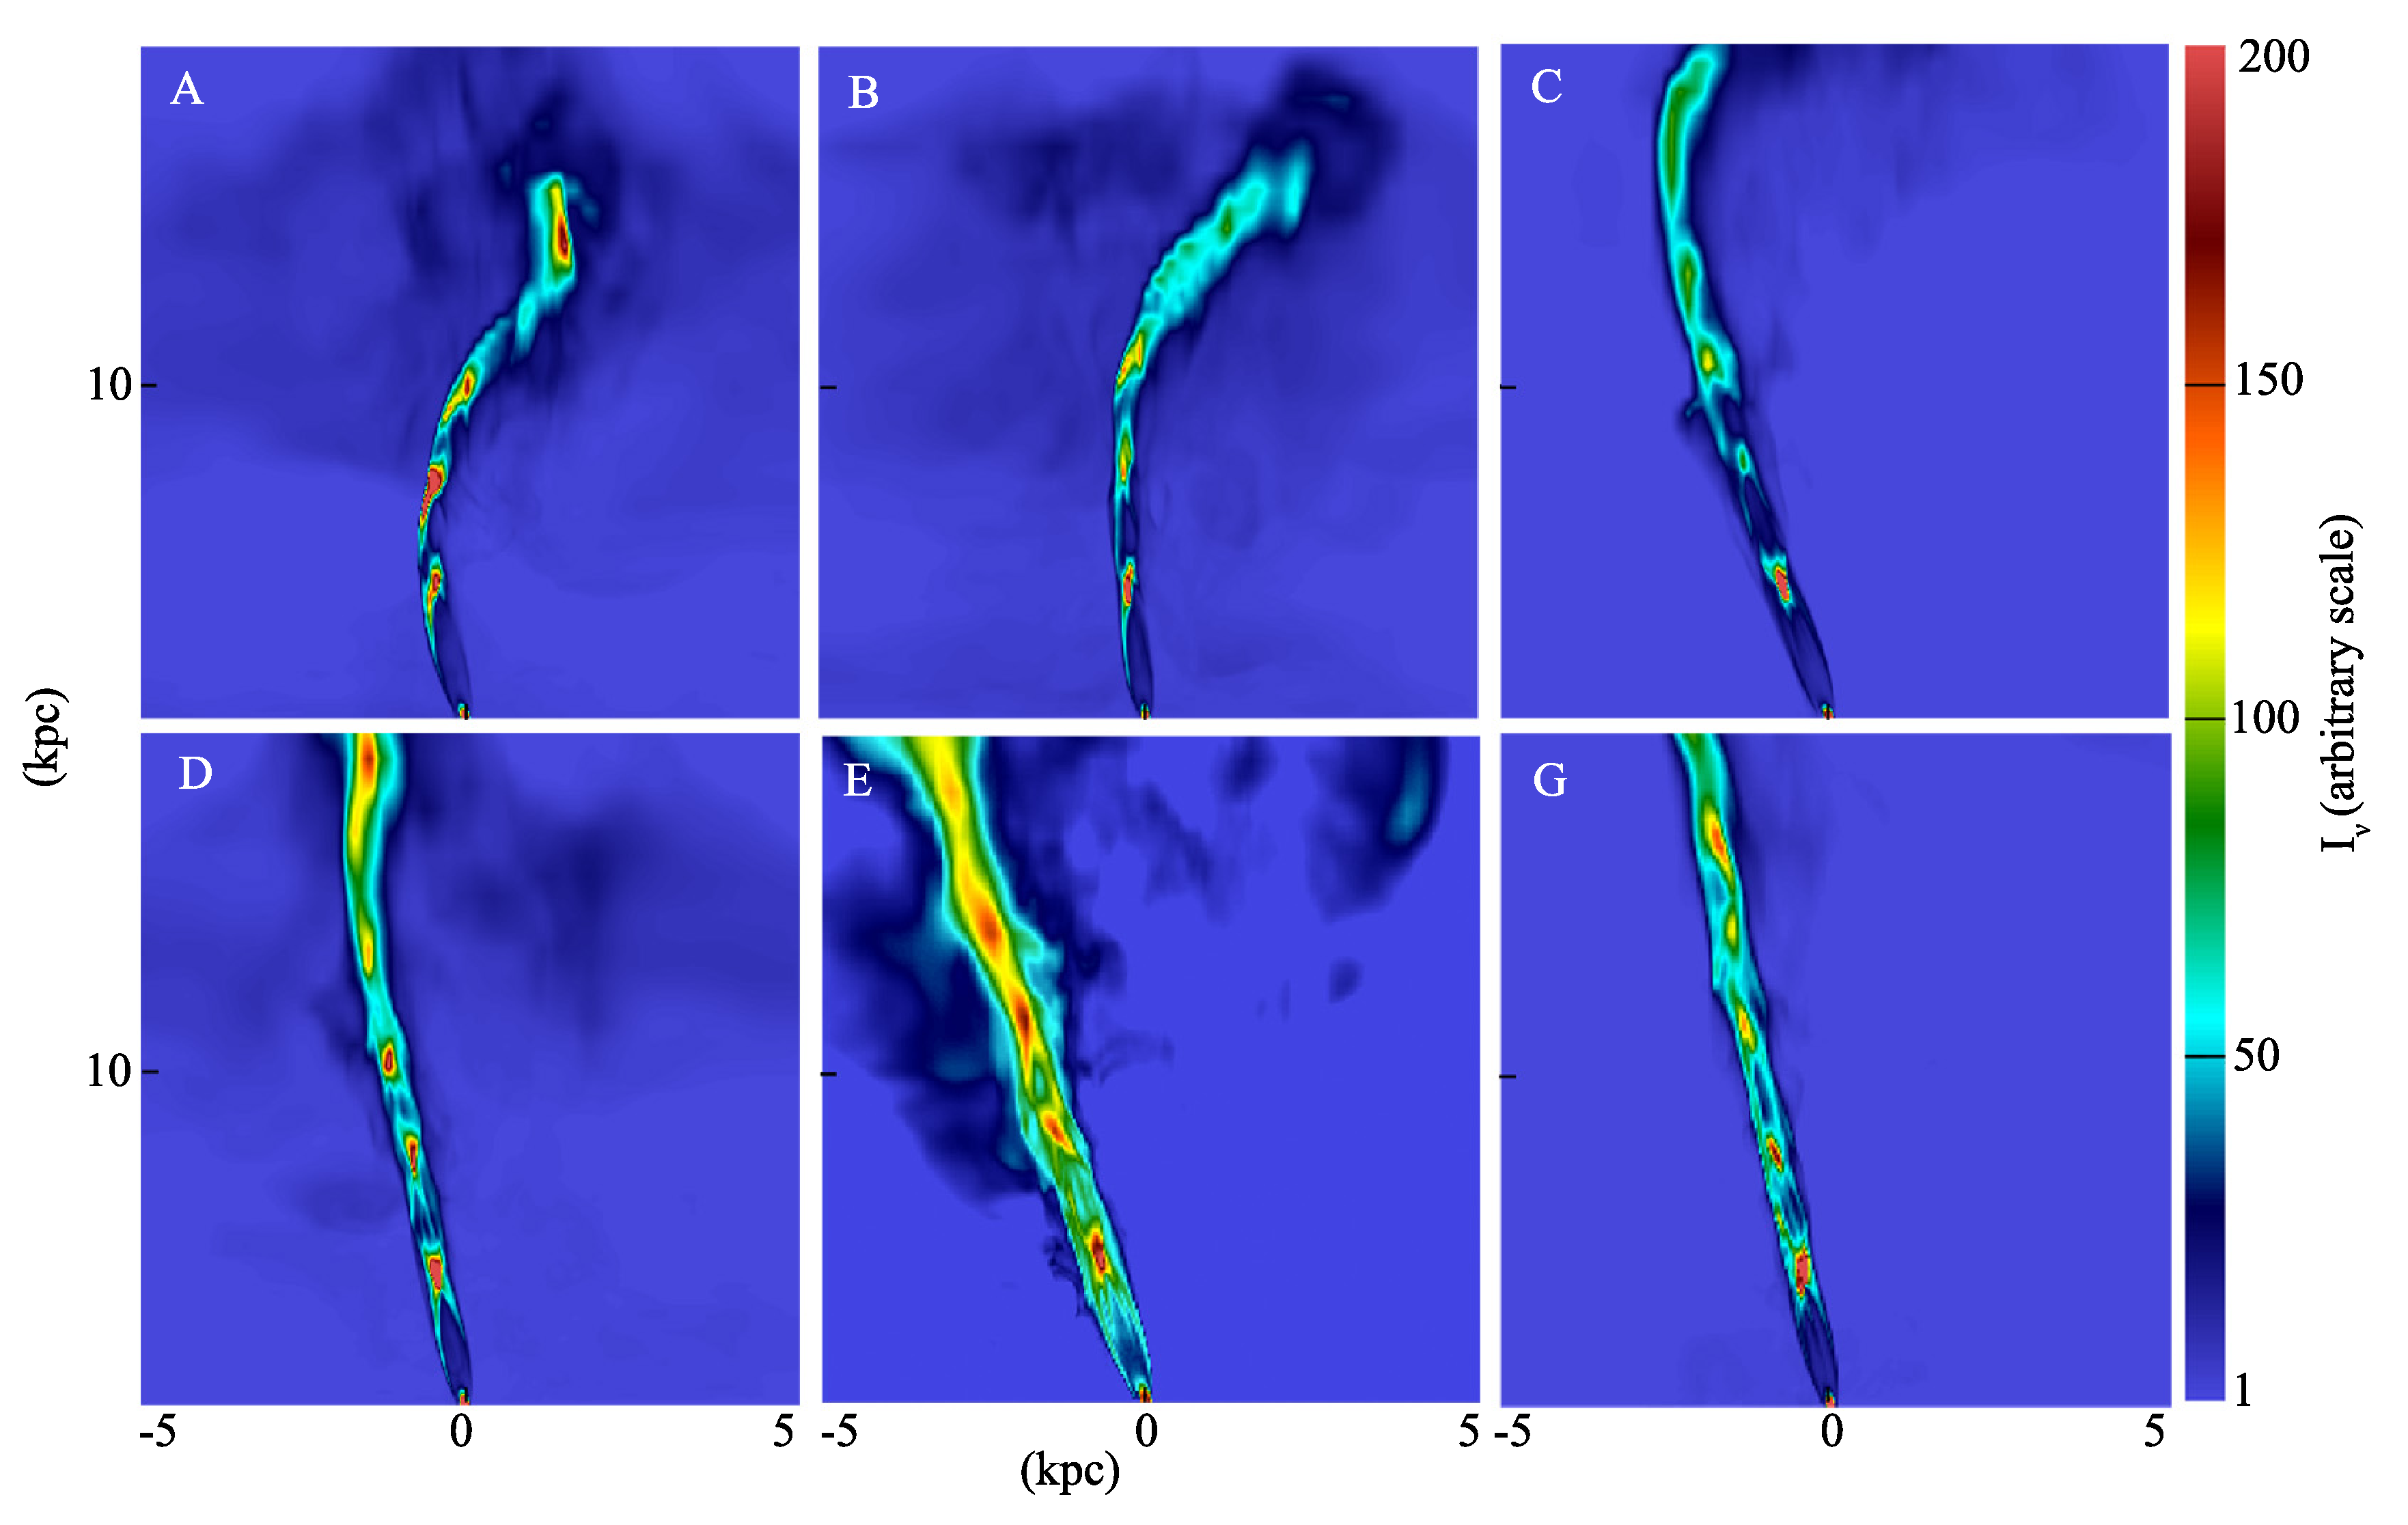
\includegraphics[width=\textwidth]{fig4.eps}
\caption{Synthetic surface brightness of models A, B, C, D, E and G. The snapshots are chosen for a simulation time at which the jet is fully developed in the computation domain. }
\label{f:cur}
\end{figure*}

Our aim is to match the simulated jet curvature within 10~kpc from the core to the observed curvature of  the Hydra A northern jet. Fig.~\ref{f:cur} shows the synthetic surface brightness images for models A, B, C, D, E, and G. The snapshots are taken when the jet is fully developed in the computational domain.
%aln
Since we are comparing the curvatures of jets with different parameters all images in Fig.~\ref{f:cur} are produced for $\theta = 90^{\circ}$.

In Fig.~\ref{f:cur} we see that the curvature of the jet increases as the precession period decreases. Models with longer precession periods produce straight jets within the first 10~kpc. For example, jets produced by the models C, D, E, and G with precession periods 5, 10, 15 and 25~Myr are straight in the inner 10~kpc. The jet with a precession period 1~Myr and a precession angle 15$^{\circ}$ is also nearly straight within this region. We see a mild curvature inside 10~kpc for model A with a precession period 1~Myr and a precession angle 20$^{\circ}$. This curvature is comparable to the curvature of the Hydra A northern jet. Therefore, on the basis of this curvature comparison alone, model A is our best match for Hydra A. This choice is confirmed by other observational features reproduced by the model. In particular, in model~A, we notice that no further knots are produced downstream of the fourth knot. However models with longer precession periods produce more than four bright knots along the jet axis. 

\subsection{Bright knots and the turbulent transition of the jet}
\begin{figure*}
\centering
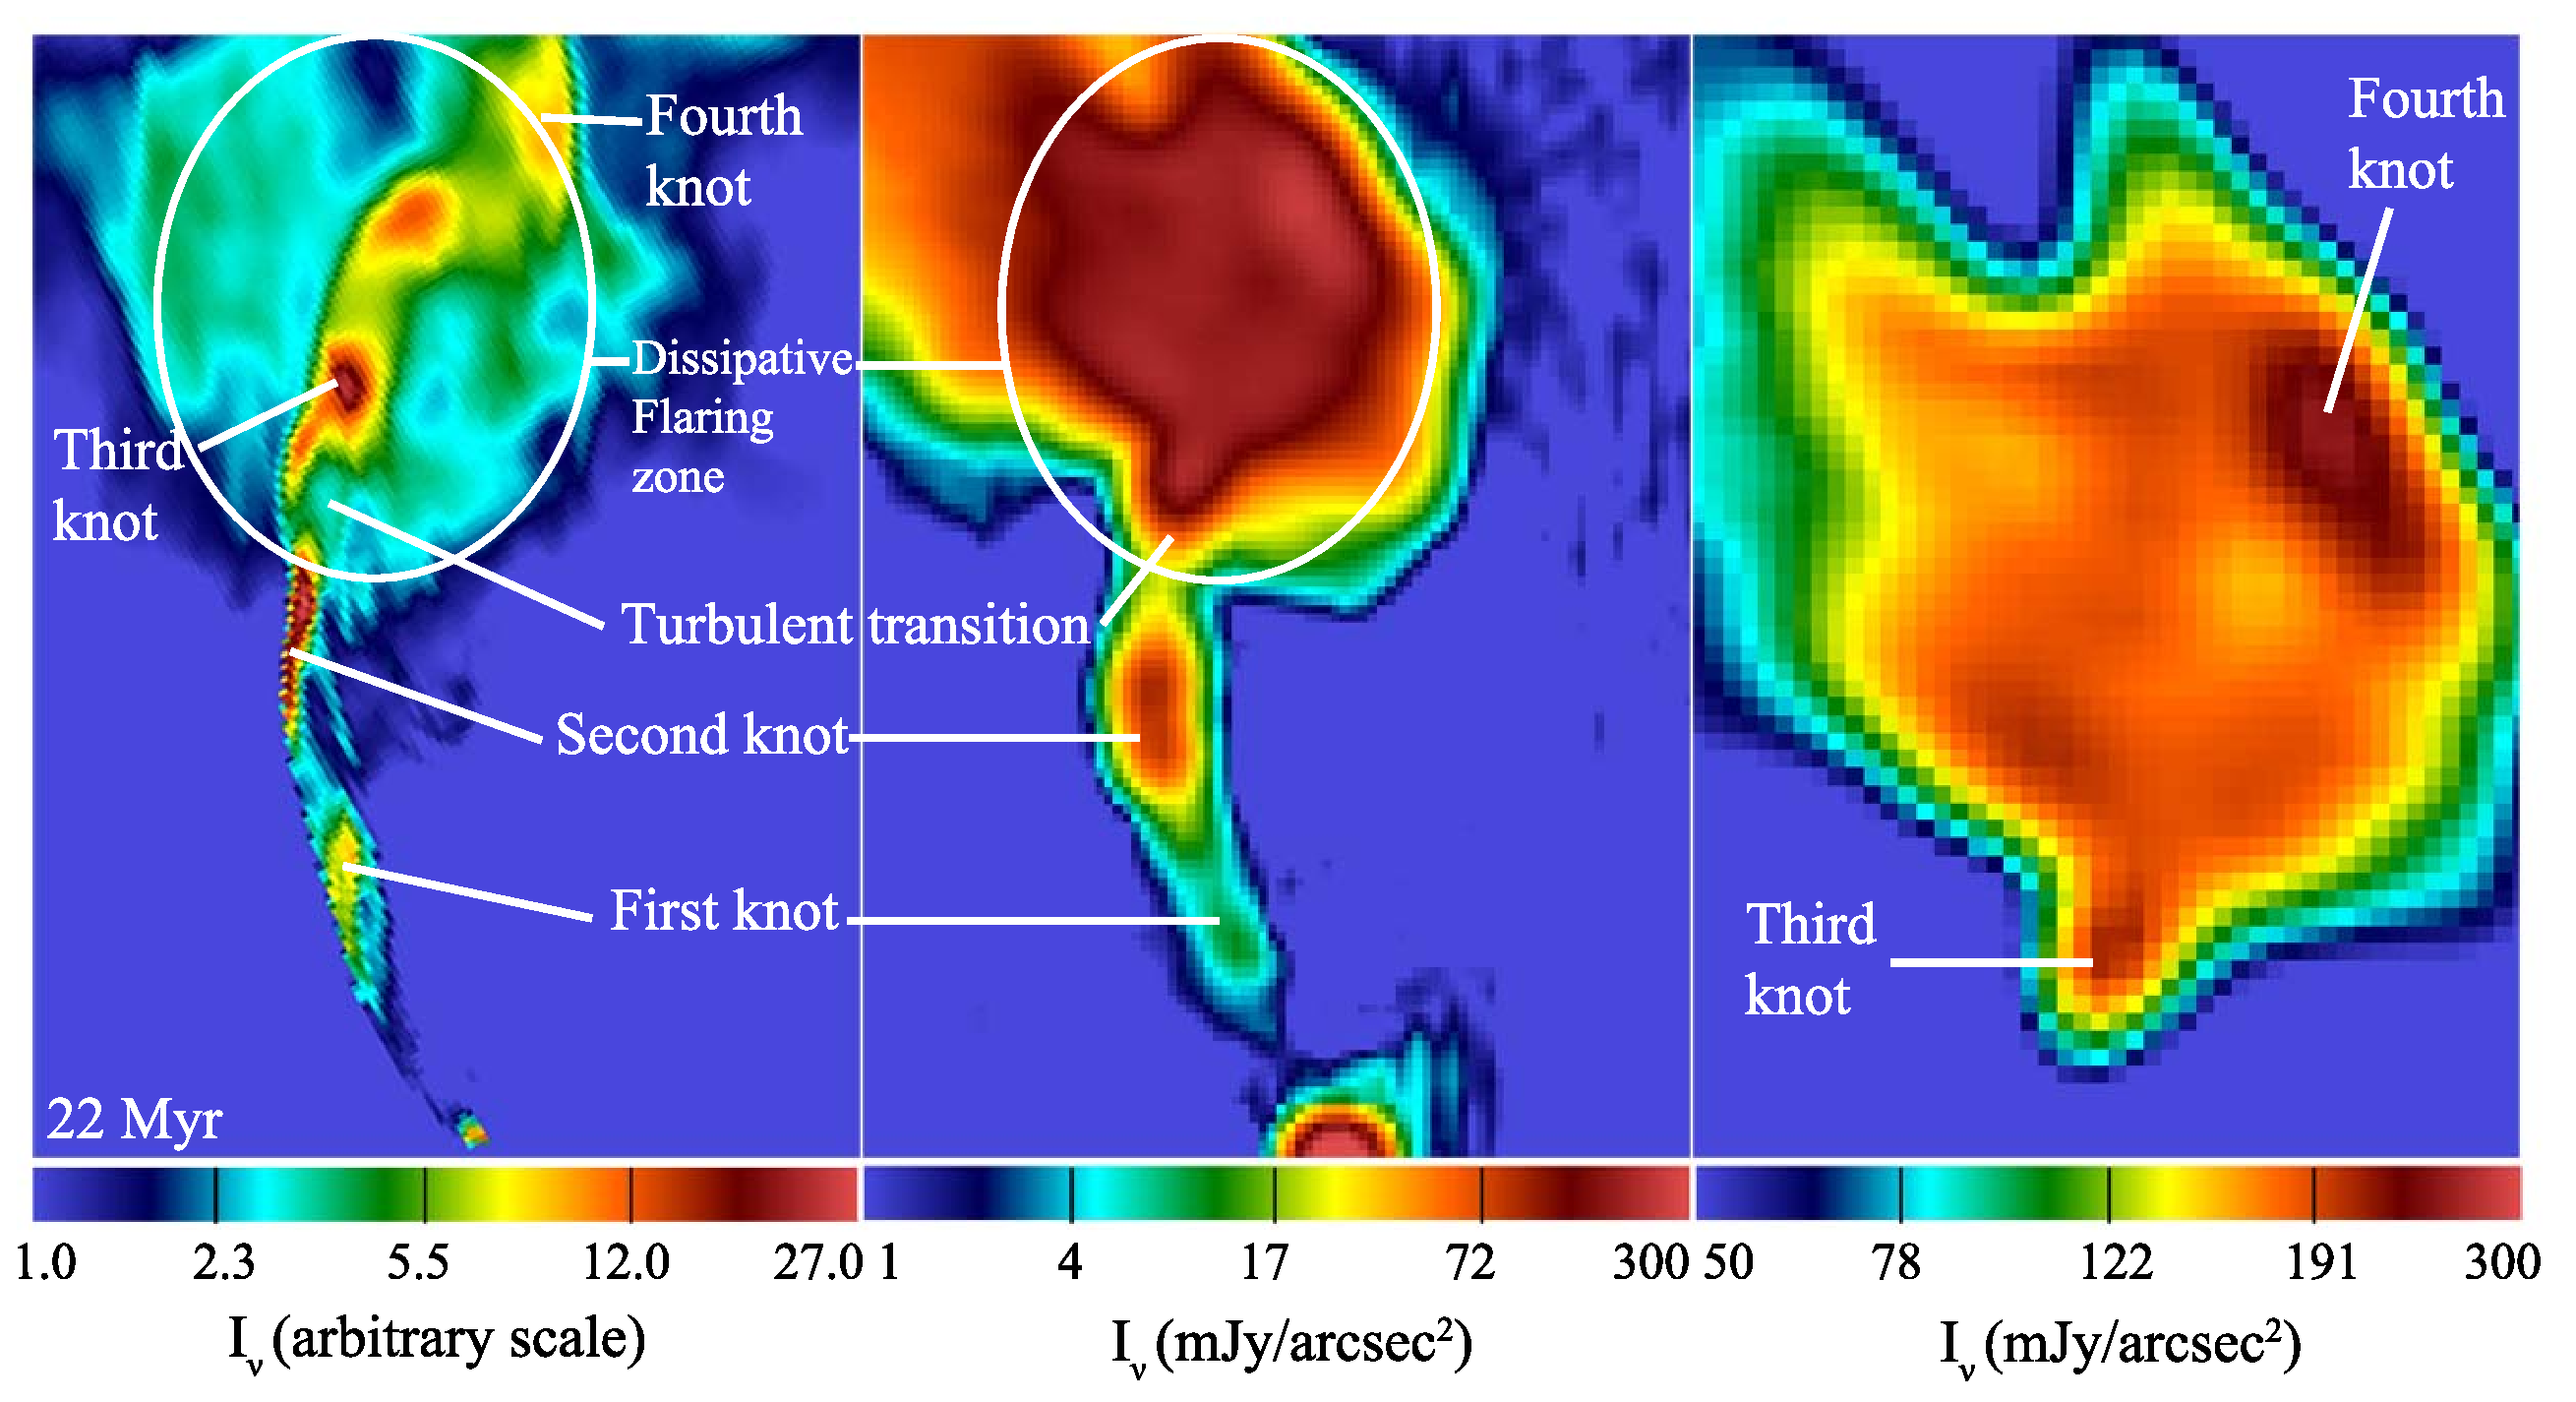
\includegraphics[width=\textwidth]{fig5.eps}
\caption{ A comparison between the source morphology of the best match model (run A, left panel) and the observational data by \citet{taylor90} (middle and right panel).}
\label{f:hyd}
\end{figure*}

\begin{figure*}
\centering
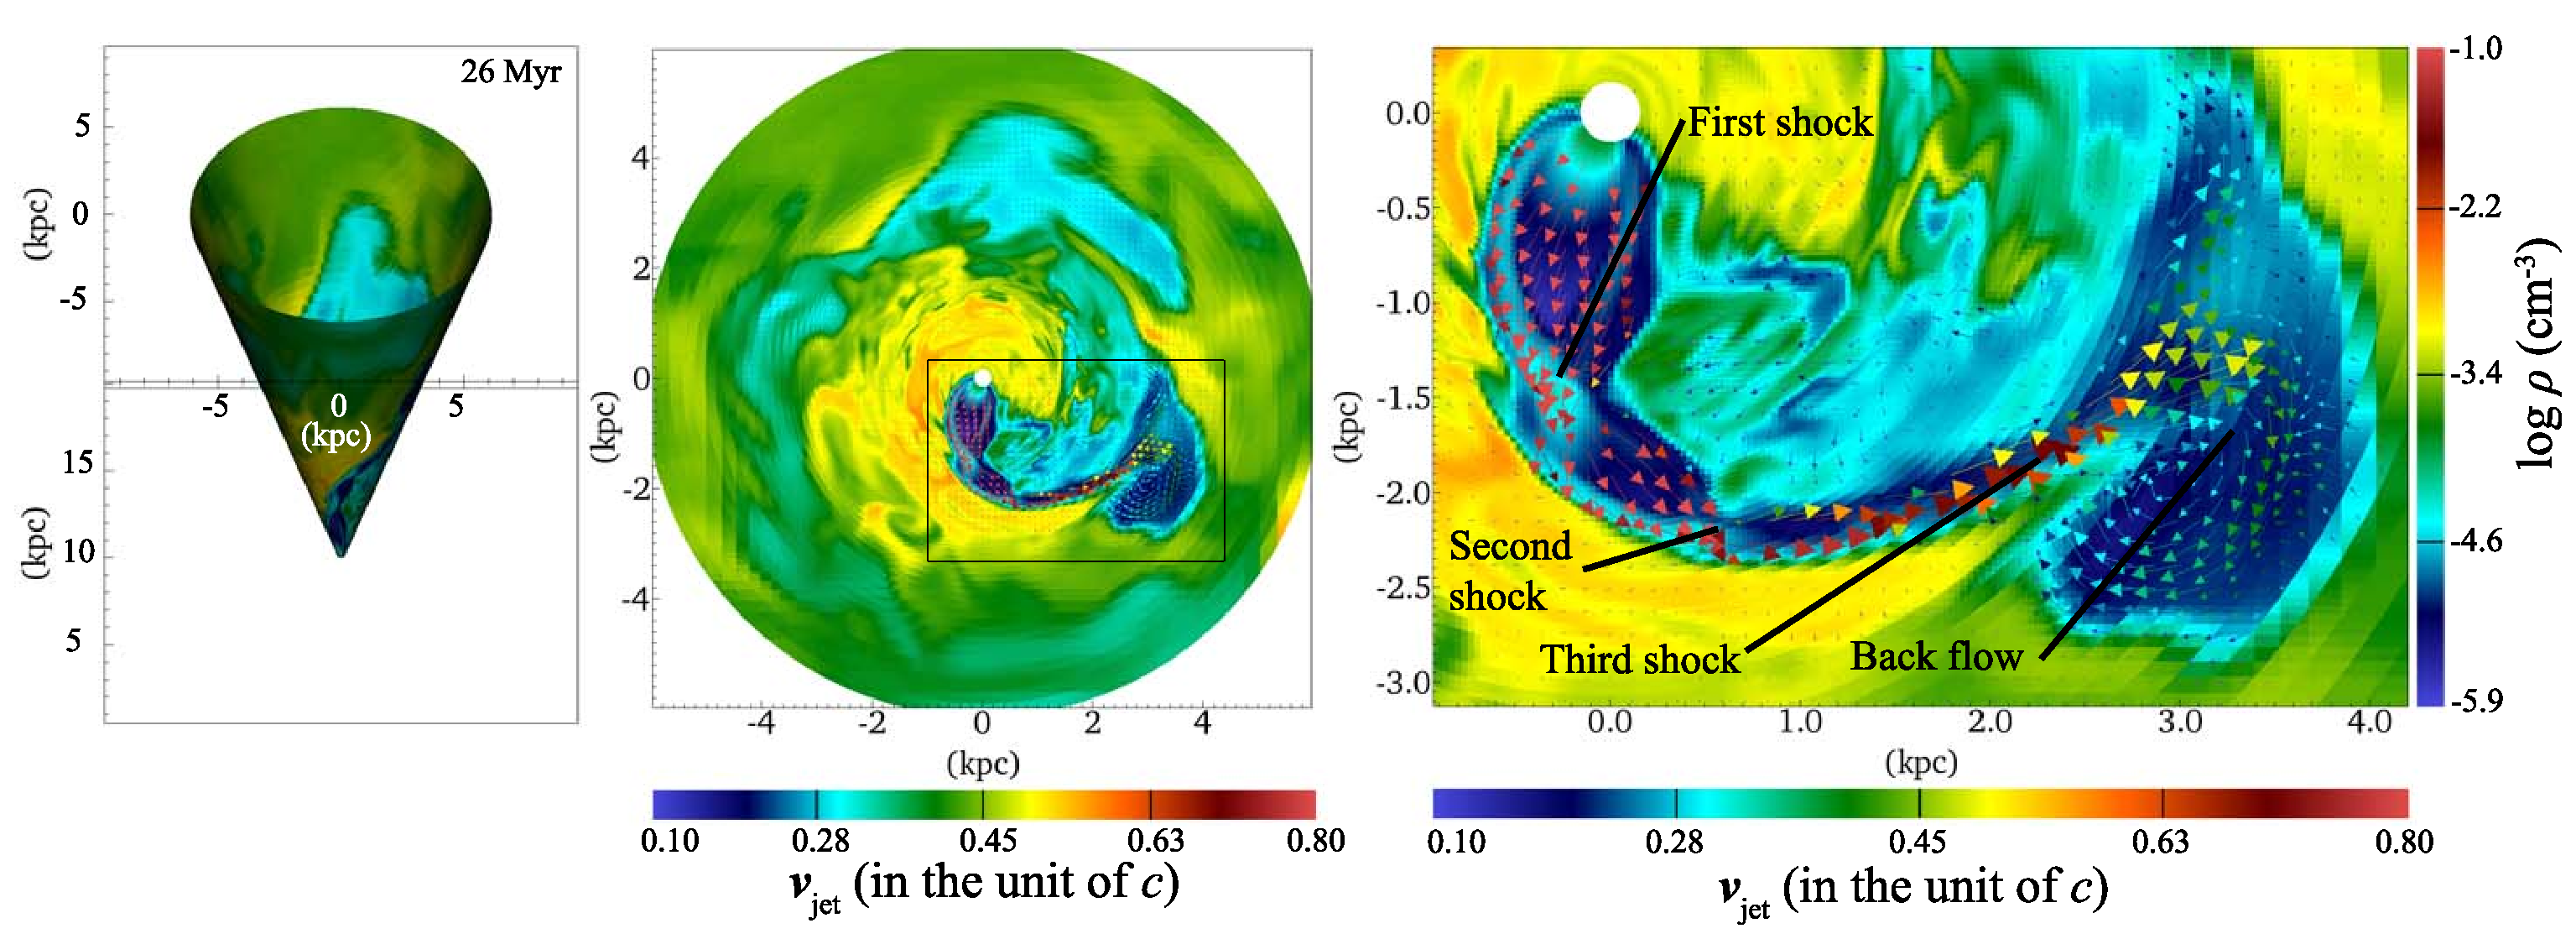
\includegraphics[width=\textwidth]{fig6.eps}
\caption{ Conic slice (cone angle 17$^{\circ}$ and cone axis aligned with the $z$-axis) of the logarithmic density image overlaid with the flow vector of the optimal model (model A) at a simulation time 26 Myr (left panel). The middle panel shows the projection of the cone onto the $x-y$ plane. The right panel is a zoom in image of the region marked by a rectangle in the middle panel.  }
\label{f:fdir}
\end{figure*}

Fig.~\ref{f:hyd} compares our optimal view of the simulated jet of model A (left panel, at a simulation time 22 Myr) and the Hydra A northern jet (middle and right panel). It is evident that the simulated jet successfully reproduces the following key features and processes occurring in the the source within the central 20~kpc. 

The moderately over-pressured precessing jet interacts with the ambient medium and produces four reconfinement shocks at approximately 4.0~kpc, 7~kpc, 10.0~kpc and 14.0~kpc from the core. Since the synchrotron emissivity is $j_{\nu} \propto p^{(3+\alpha)/2}$, downstream of the reconfinement shocks the pressure and therefore the surface brightness increase producing four bright knots. We see that the locations of the bright knots produced with this model agree well with the locations of bright knots in the Hydra A northern jet located at approximately 3.7~kpc, 7.0~kpc, 11.0~kpc and 16.0~kpc (deprojected) from the core and shown in the middle and right panel. In the simulated jet we see that a turbulent transition of the jet to a plume occurs approximately after the second bright knot, which is consistent with the observations. This figure also shows that in the optimal model, the turbulent jet starts to forms a dissipative flaring zone (marked by the ellipse in the left panel). This is the beginning of a large plume structure as observed in the Hydra A northern jet. Currently, we are investigating further development of the plume for an extended inner region (up to ~30kpc) of the northern jet with high resolution simulations. This will be presented in our next paper.

In the Hydra A northern jet, the flaring region within approximately 11 to 20~kpc where the plume starts, is very bright compared to the inner collimated jet. The corresponding region in our optimal model does not reach the same level of brightness. However, the flaring region is strongly turbulent (see \S~\ref{flaring}).
The amplification of the magnetic field resulting from this turbulence may be responsible for this dramatic increase of the source brightness. Since, our model is purely hydrodynamic and the amplification of the magnetic field is not reflected in the synthetic brightness images. In order to produce more accurate synthetic brightness images magnetohydrodynamic (MHD) models are required. Therefore, further development of this model with the inclusion of magnetic field would be interesting. 

\subsection{Turbulent flaring zone}
\label{flaring}
Fig.~\ref{f:fdir} shows the logarithmic density of run A (at a simulation time 26 Myr) sliced by a cone with a cone angle of 17$^{\circ}$ (left panel) and cone axis aligned with the precession axis ($z$ axis). To obtain a clear view of the jet and the flow direction the cone is projected onto the $x-y$~plane (right panel of Fig.~\ref{f:fdir}) and overlaid with the flow vectors. A zoom in of the region marked by a rectangle in the middle panel is shown in the right panel. It is noted here that, although the precession angle in model A is 20$^{\circ}$, the jet is mostly visible along the conic slice with a cone angle 17$^{\circ}$. This is the result of the reflective boundary condition at the lower $z$ boundary. The reflection of the back flow on the side of the jet closest to the boundary pushes the jet towards the precession axis. Therefore, the jet is maximally visible along a conic slice with cone angle less than $20^{\circ}$. 

In Fig.~\ref{f:fdir} we see that after the turbulent transition of the jet some jet plasma hits the dense cocoon plasma and produces a strong back flow (shown in the right panel). This turbulent back flow  establishes a flaring region. Such a flaring region of the jet is apparent at approximately 10 to 20~kpc from the core in the northern jet of Hydra A.
 Moreover, in the polarisation image of Hydra A \citep{taylor90} we see that the polarisation significantly falls from 40$\%$ (in the collimated jet) to 10$\%$ in the flaring region. This reduction in polarisation suggests that the flaring region of the northern jet is turbulent, which is consistent with our simulations.  

%%%%%%%%%%%%%%%%%%%%%%%%%%%%%%
%
%			Forward shock
%
%%%%%%%%%%%%%%%%%%%%%%%%%%%%%%
\subsection{Forward shock} 
\begin{figure*}
\centering
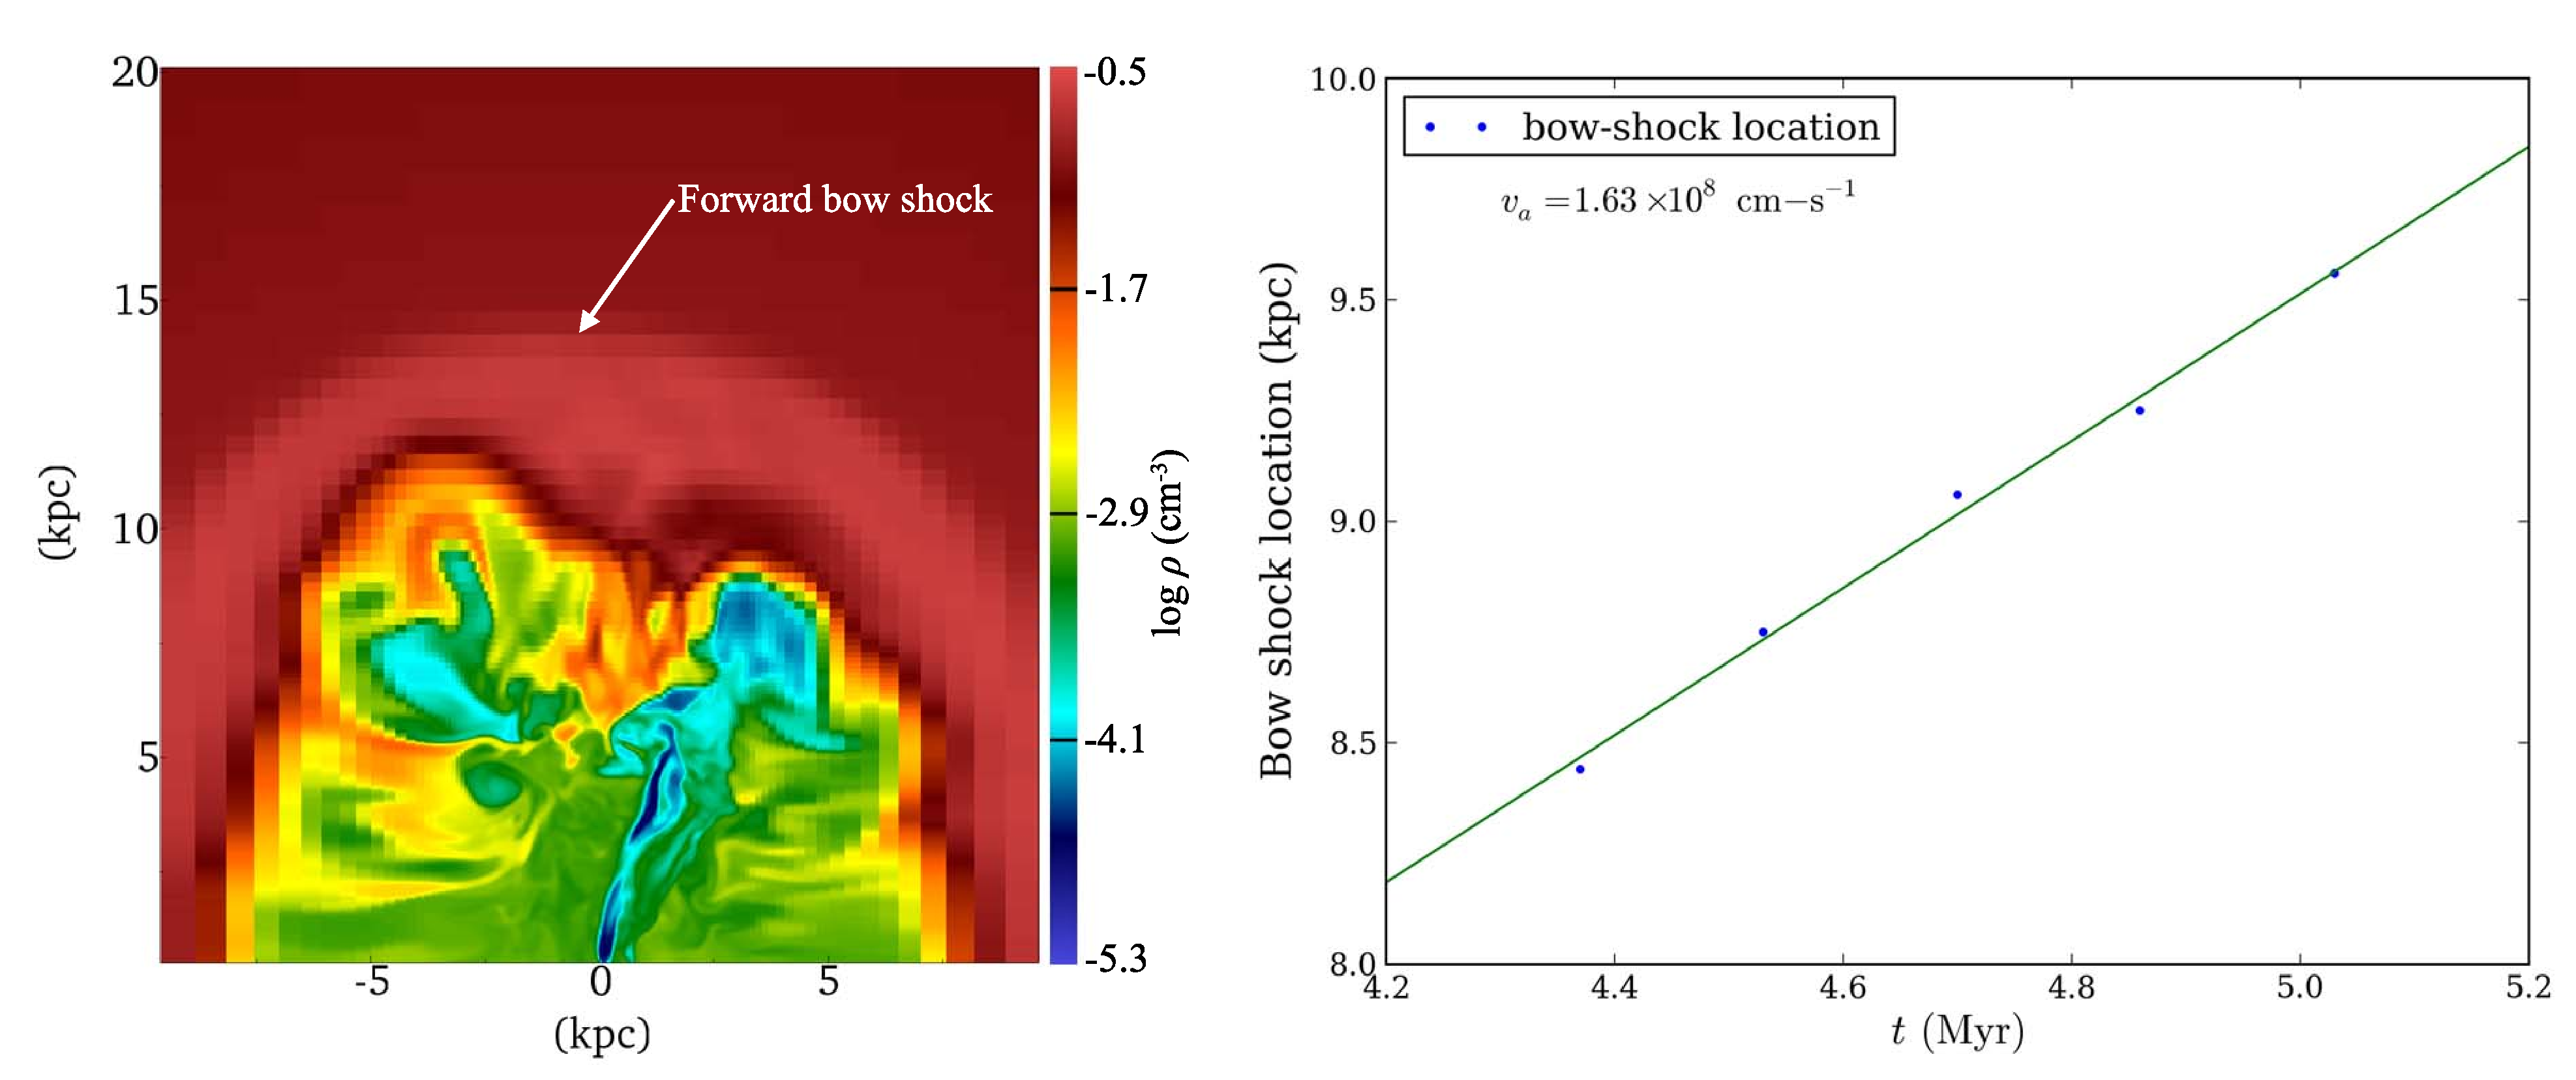
\includegraphics[width=\textwidth]{fig7.eps}
\caption{ Left: Midplane slice of the logarithmic density snapshot of model A. The forward bow shock is marked by an arrow in this panel. Right: Locations of the forward shock at five different time steps (points) . A least square linear fit (line) gives a shock advance speed $\approx$ 1630 km s$^{-1}$. }
\label{f:fsh}
\end{figure*}
%GVB
%In our best natch model the cocoon is separated from the ambient medium by an advancing forward shock. Here we estimate the Mach number of that forward shock. 

In our optimal model the radio jet-ICM interactions are bounded by an advancing forward shock. Here we estimate the Mach number of that forward shock. 

The forward bow shock is shown in the logarithmic density snapshot of model A (left panel of Fig.~\ref{f:fsh}). In the right panel of Fig.~\ref{f:fsh} the location of the forward shock along the $z$-axis at five different time steps is traced by points. Fitting a least square line to the shock locations we obtain shock advance speed $\approx  1630$ km s$^{-1}$ of the forward shock. The sound speed at approximately 15~kpc from the core is $\approx 880$ km s$^{-1}$. Hence, the Mach number of the forward shock is $\approx 1.85$. 
There is a mild pressure jump $\approx 3.4$ at the forward shock. The low Mach number and mild pressure jump indicate that the heating of the atmosphere by the radio AGN in its earlier stage is gentle. This general feature of the heating of cooling flows was inferred by \citep{mcnamara12}. 

%%%%%%%%%%%%%%%%%%%%%%%%%%%%%%
%
%			Mis-aligned knot
%
%%%%%%%%%%%%%%%%%%%%%%%%%%%%%%
\subsection{Misaligned bright knot}
\begin{figure*}
\centering
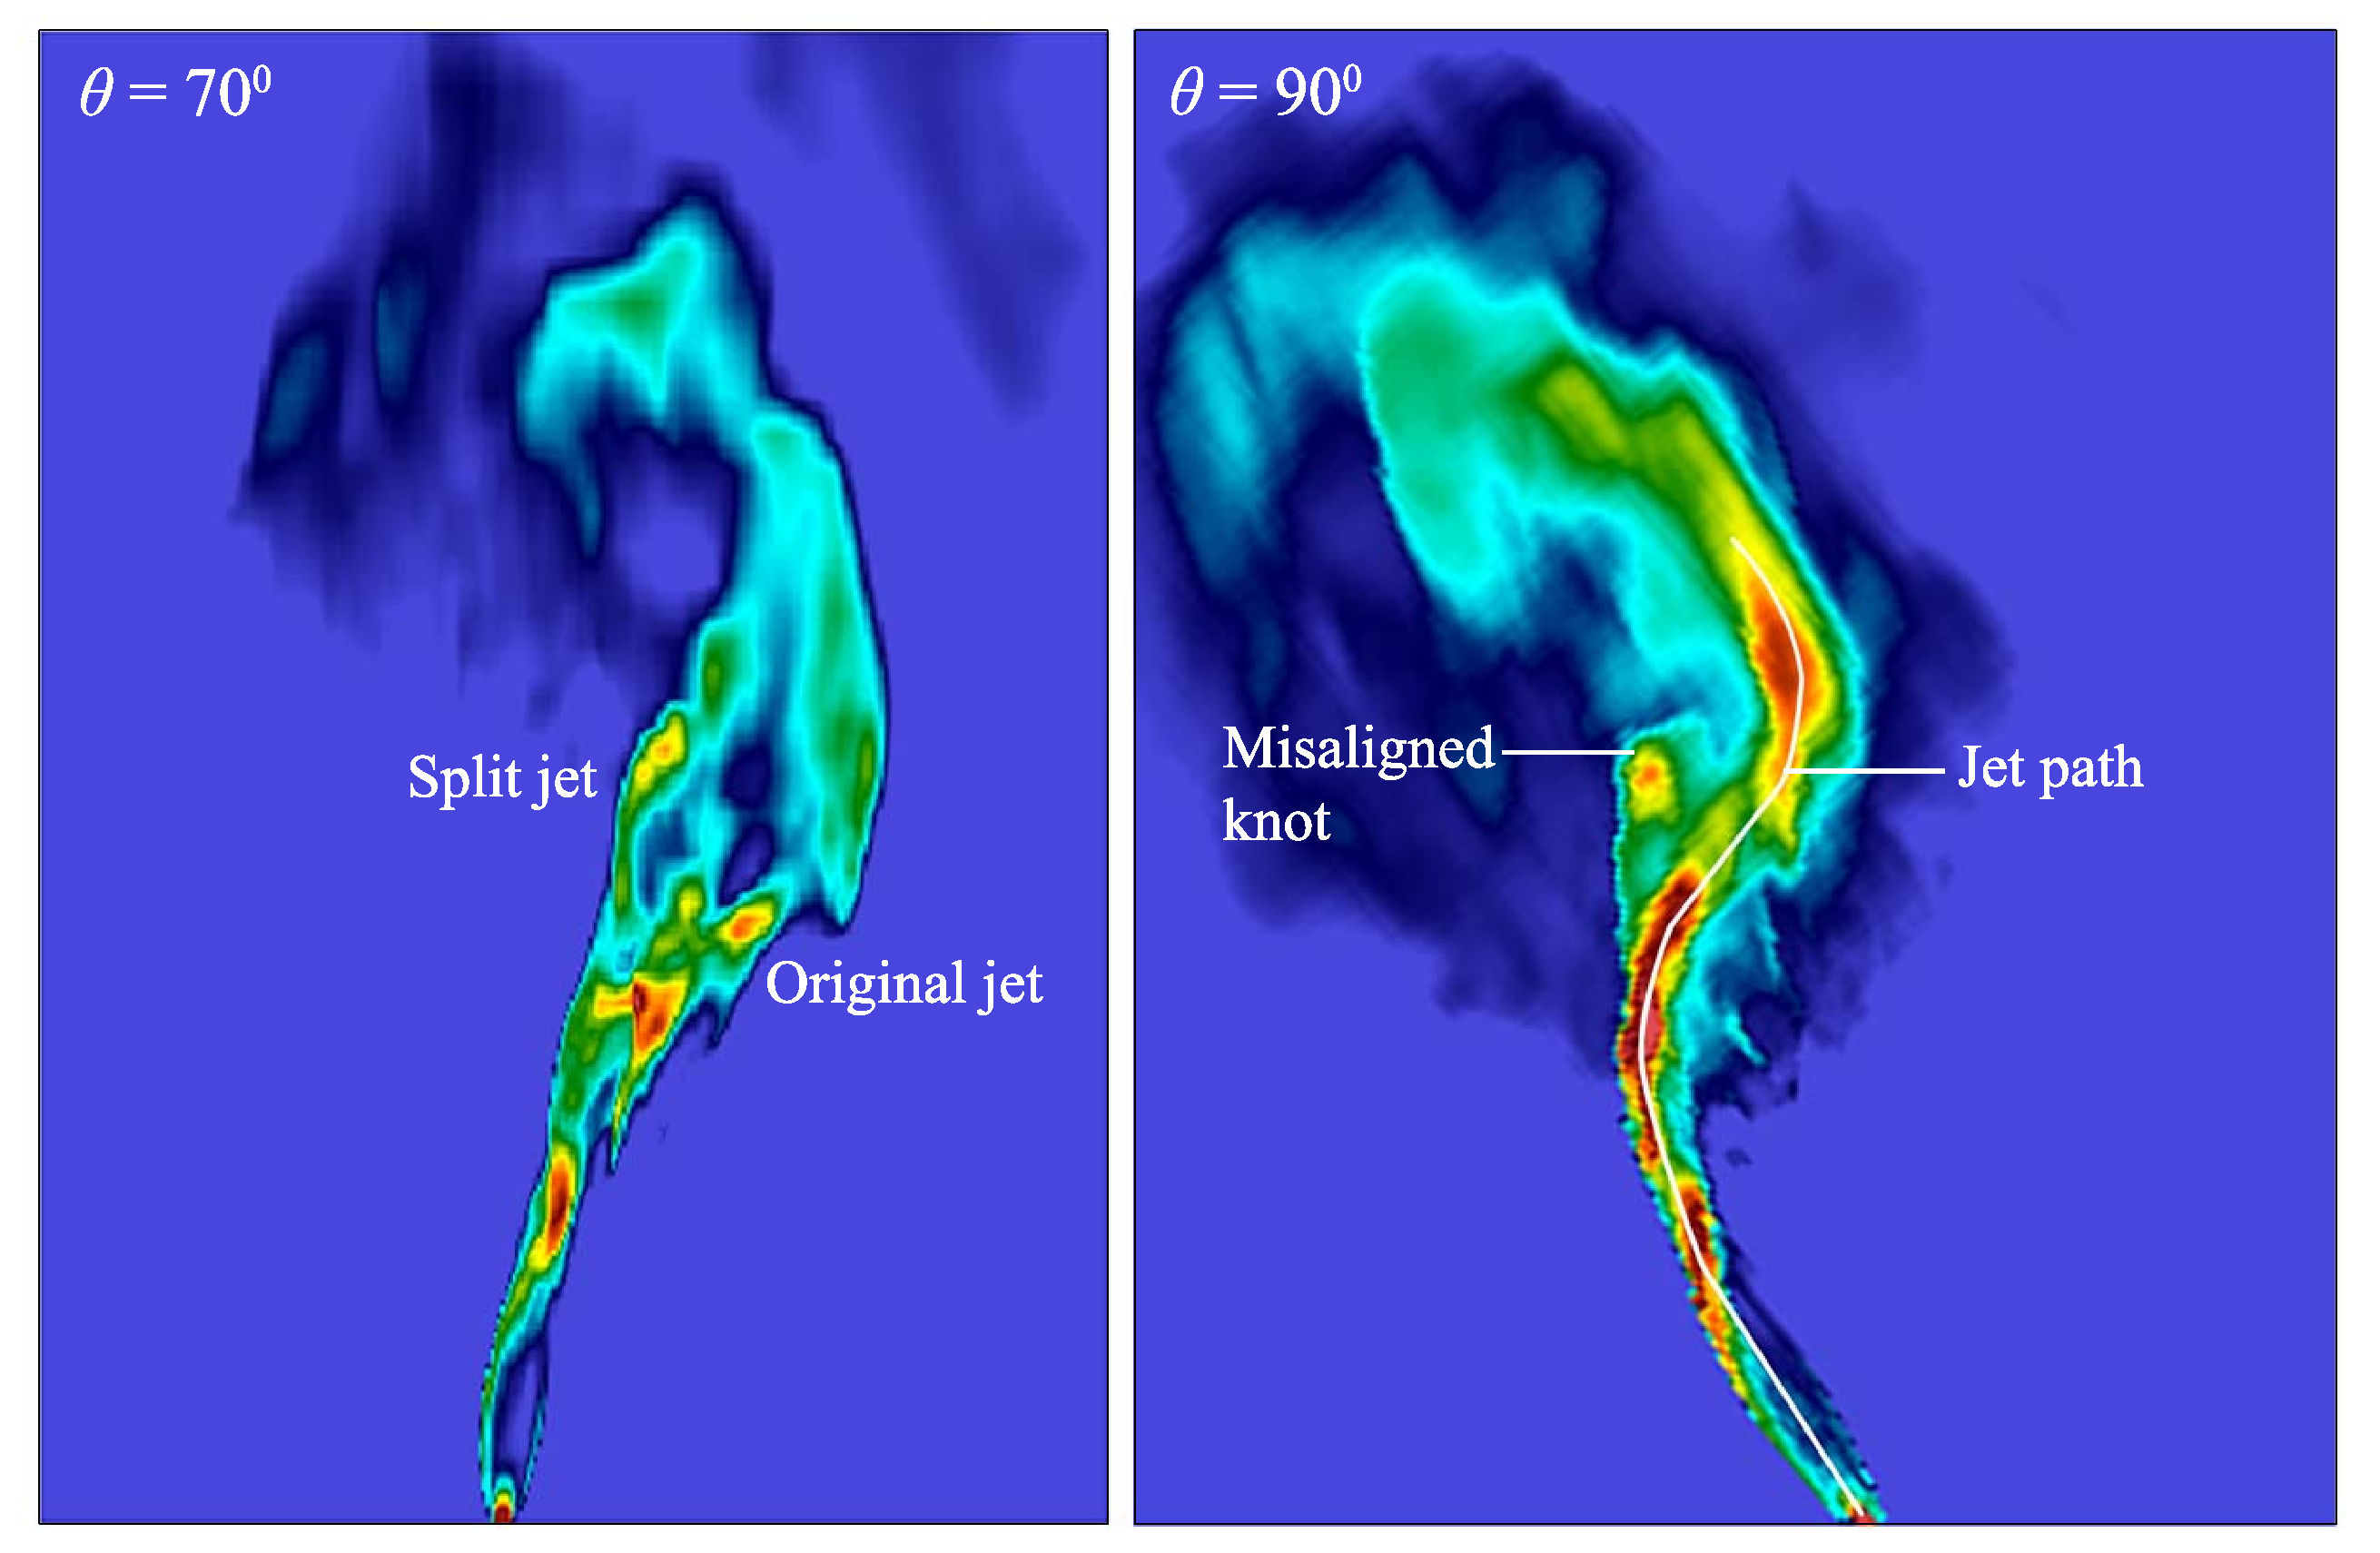
\includegraphics[width=\textwidth]{fig8.eps}
\caption{A misaligned knot produced by the jet splitting. In the left panel the jet splitting is shown in a synthetic surface brightenss image for a line of sight $\theta = 70^{\circ}$. In the right panel the synthetic surface brightness image is presented for a different line of sight $\theta = 90^{\circ}$, for which the jet path and the misaligned knot are clearly shown. }
\label{f:mknt}
\end{figure*}

In the turbulent flaring region of the Hydra A northern jet there is a  knot, which is not aligned with the main trajectory of the jet. This mis-aligned knot is approximately two kpc north of the third knot and is marked as 'misaligned knot' in Fig.~\ref{f:obs}. This knot is formed as a consequence of the transition to turbulence of the jet. The jet temporarily splits in two forming the misaligned knot and then returns to its final trajectory through the plume region (see Figure~\ref{f:mknt}). This happens only with our optimal model (A).

%Mis-aligned knots appear frequently in synthetic surface brightness images of our best matching model (run A). Models with higher precession periods (run C, D, E, F and G), and model with precession period 1~Myr but low precession angle (run B) do knot produce such mis-aligned knot. The mis-aligned knot usually appear in the flaring region of the jet and are short-lived  compared to the first couple of knots in the main jet at smaller radii. Close inspection of the flow evolution reveals that the jet occasionally splits in two - a main jet and a secondary jet, with the mis-aligned knot forming as a reconfinement shock in the secondary jet. Surveying the surface brightness image evolution of our simulations from a given line of sight, we find that jet splitting and the formation of mis-aligned knots occurs about 2 to 4 times per precession period. It is possible that the occurrence frequency is higher if we included counts along different lines of sights. The splitting of the jet always occurs near the region where the flow transitions to turbulence, and is often in the shape of a tuning fork. We can see that the mis-aligned knot is due to a reconfinement shock because the jet flow remains continuous along the split jet with knots forming at roughly the same distance from the fork. 
%
%The morphology of the split jet with reconfinement shocks forming in both the primary and secondary jet is sketched in panel 1 of Fig.~\ref{f:mknt}. The second and third panels of Fig.~\ref{f:mknt} show a snapshot example from model A (t = 26~Myr) at viewing angles of $\psi=70$ and $\psi=90$ respectively, in which the jet is split and has created two knots, one aligned with the precessional trajectory of the jet, and one clearly offset northward from the main jet. In Appendix~\ref{A:mknt}, we show further examples of the splitting of the jet and the formation of a mis-aligned knot, all at different snapshots from the model A.
%
%The reason for the splitting of the jet is difficult to pin down. Even the exact geometry of the splitting is difficult to reconstruct. We cannot easily determine the orientation of the splitting (i.e., the plane of the ``tuning fork''). Some snapshots of our simulations appear to indicate that the splitting occurs perpendicular to jet along the direction of precession (e.g. panels 2 and 3 Figure ??), In this case, the leading edge of the precessing jet, whose shocked region (region A in panel 1 of Fig.~\ref{f:mknt}) is highly overpressured, is perturbed, allowing the jet to channel, expand, and reconfine in a different direction to the original jet. Due to the incoming flow that compresses the shocked region at the leading edge of the precessing jet, that side is more overpressured than the shocked region of the receding edge (region B in panel 1 of Fig.~\ref{f:mknt}). The leading edge is also more exposed to perturbations as the precessing jet  moves into regions of turbulent backflow. A small blob of slightly denser gas back-flowing into the path of the jet would easily split the jet. This could naturally explain why we often see the split secondary jet emerge from the leading edge of the precessing primary jet. As the primary jet catches up with the split secondary jet, the latter is seen to evolve into the primary jet, while the other jet and its associated knot fades.
%
%The fact that the secondary jet evolves into the primary jet  may also suggests that jet  splitting and the formation of misaligned knots could, in fact, be a manifestation of jet jittering, helical bending of the jet caused by the Kelvin-Helmholtz shear instability \citep{begelman84, hardee13}. The bending would only be temporary because the jet flow keeps re-establishing itself as it precesses to propagate in a different direction. Alternatively, the appearance of knots may simply be related to transition to turbulence giving rise to random bifurcations to the flow direction of the marginally laminar jet. 

%%%%%%%%%%%%%%%%%%%%%%%%%%%%%%%%%%%%%%%%%%
%
%				Implication of precession
%
%%%%%%%%%%%%%%%%%%%%%%%%%%%%%%%%%%%%%%%%%%
\subsection{Implication of precession: Estimate of viscosity parameter of the AGN disk}
Knowledge of the precession period of the jet provides us with information that can be used to estimate the well known accretion disk viscosity parameter $\alpha$. A black hole (BH) whose spin is misaligned with the angular momentum of the accretion disk aligns the surrounding inner part of the disc to the BH spin axis via Lense-Thirring precession and internal viscosity up to a critical radius known as the Bardeen-Petterson radius, $r_\mathrm{BP}$ \citep{bardeen75}. Beyond $r_{\rm BP}$, the disk retains its original structure because of its dominant angular momentum. Viscous torques in the outer accretion disk force the spin axis of the black hole to precess until it is aligned with the angular momentum of the outer disk \citep{rees78, scheuer96, natarajan98, caproni07}. The alignment time-scale can be considered equivalent to the precession period of the jet. Using the alignment timescale, a jet precession period $\approx$ 10$^8$-10$^{10}$ yr has been estimated for the source, NGC 4258 \citep{caproni07}. 

We use the theory of \citet{natarajan98} to estimate the accretion disk viscosity parameter $\alpha$. Let $t_{\rm align}$ be the alignment time-scale, $a$ the spin parameter of the black hole, $\alpha$ the viscosity parameter of the accretion disk, $L$ the total power provided by the black hole,
%($L_{\rm bol}$ + $L_{\rm jet}$), where $L_{\rm bol}$ is the bolometric luminosity of the source, and $L_{\rm jet}$ is the jet kinetic power 
$L_{\rm E}$ the Eddington luminosity, $M_{\rm BH}$ the mass of the black hole, $M_{\odot}$ the solar mass, and $\epsilon$ the accretion efficiency of the black hole. Then, from the equation for the alignment time of the black hole (\citealt[][equation 2.16]{natarajan98}) we obtain:
\begin{align}
\alpha & = 0.04 \left(\frac{a}{0.8}\right)^{-11/26} \left(\frac{L}{0.02 L_{\rm E}}\right)^{7/13} \\ \nonumber 
           & \times \left(\frac{M}{ 10^9 M_{\odot}}\right)^{1/26}  \left(\frac{\epsilon}{0.1}\right)^{-7/13} \left(\frac{P}{\rm Myr}\right)^{8/13}\:.
\end{align}
where $P(=t_\mathrm{align}$) is the precession period of the jet.

The mass of the supermassive black hole in Hydra A is approximately $10^9$ M$_{\odot}$ \citep{fujita13}. The total jet power provided by the black hole is $L=2L_{\rm jet}\approx 2 \times 10^{45}$ erg s$^{-1}\approx 0.02L_{\rm E}$. Using $\epsilon = 0.1$, $P=1$~Myr, and a range of $a$ (= 0.1 to 1) we obtain $0.03\le \alpha \le 0.15$. The upper end of the range of $\alpha \approx 0.15$ (for $a \approx 0.1$) is consistent with the range of values typically inferred from observations of dwarf novae $0.1\le \alpha \le 0.4$ \citep{king07}.

However, in general, there is a discrepancy between values of $\alpha$ derived from observations and those derived from numerical magneto-hydrodynamic (MHD) simulations; the later are generally an order of magnitude lower than the former. For instance, the quasi-steady disk MHD models by \citep{parkin13b} imply $\alpha \approx 0.04$. Such a low value is consistent with the lower bound of our estimate of $\alpha$ (for $a\approx 0.9$). The lowest value $\alpha = 0.03$ in the range is consistent with the estimates by \citet{starling04} from observations of AGN disks.

\noteA{New paragraph below, heavily borrowed from Brian's email comments}
The jets in Hydra A are being launched from within a rotating disk or ring of ionized gas, molecular gas and dust, with the jet axis slightly inclined with respect to the disk’s angular momentum axis \citep[see, e.g.,][and references therein]{hamer2014a}. The inclination angle of the disk with respect to the jet is similar to the precession angle we infer. The kpc scale molecular disk, which is forming stars \citep{mcnamara1995a}, may ultimately be the fuel supply for future episodes of jet activity. For the current jets, the settling time of the gas in the disk is too long and is competing with consumption by star formation. Nevertheless, the relationship between the disk and jet geometry is compelling.


%%%%%%%%%%%%%%%%%%%%%%%%%%%%%%%%%%%%%%%%%%%%%%%%%%%%%%%%%%%%%%%%%%%%%%%%
% 
%												Discussion and Summary
%
%%%%%%%%%%%%%%%%%%%%%%%%%%%%%%%%%%%%%%%%%%%%%%%%%%%%%%%%%%%%%%%%%%%%%%%%

\section{Summary and Discussion}\label{s:discussion}
In Paper I we modelled the inner two bright knots of the Hydra A northern jet utilising axisymmetric straight jet simulations. In this paper we have developed that model by incorporating jet precession and studying the three dimensional interaction of the jet with the intracluster medium. Our three dimensional precessing jet model successfully reproduces the prominent features of the complex inner 20~kpc jet-lobe morphology in the northern side of Hydra A.  

We have performed a parameter space study using parameters obtained from Paper I, a range of precession periods (1, 5, 10, 15, 20 and 25~Myr) and two precession angles (15$^{\circ}$ and 20$^{\circ}$). From our parameter study we find that model A with a precession period of 1~Myr and a precession angle of 20$^{\circ}$ produces the correct jet curvature, the correct number of knots, and the jet to plume transition at approximately the correct locations. Therefore we choose this model as our best matching model. 

Our optimal model reproduces:
\begin{enumerate}
\item Four bright knots along the direction of the jet. The bright knots appear at the locations of the biconical shocks resulting from reconfinement shocks associated with recollimation of the jet by the ambient medium. The locations of the knots at approximately 4, 7, 10 and 14~kpc coincide reasonably well with the observed bright knots at approximately (3.7, 7.0, 11.0 and 16.0~kpc). 
\item The turbulent transition of the jet to a plume at approximately $9$~kpc compared to the observed transition location at 10~kpc. The initially supersonic jet is significantly decelerated by the first two reconfinement shocks and transition to turbulence begins after the second knot.  
\item A turbulent flaring zone at approximately 10-20~kpc from the core. The back flowing jet plasma from the cocoon wall near the fourth knot produces strong turbulence in this region. The turbulence is responsible for the widening of the flow at approximately 10~kpc from the core. This simulated feature is consistent with the following observed feature of Hydra A. From the polarisation image \citep{taylor90} we see that the polarisation drops from $40\%$ in the collimated jet (until 10~kpc from the core) to $10\%$ in the flared region (10-20~kpc from the core) on the northern side of Hydra A. This drop in polarisation suggests that the flaring zone (10-20~kpc from the core) could be turbulent.
\item A misaligned knot in the turbulent flaring zone. This feature is only produced in model A, supporting the choice of that model as the best match to Hydra A. 
\end{enumerate}

We estimate the Mach number of the forward advancing shock $\approx 1.85$ from our optimal model. This low Mach number and the pressure jump ($\approx 3.4$) of the ambient medium associated with the forward shock  suggest a gentle heating of the of the ICM by the radio AGN in its initial phases of evolution as noted by \citet{mcnamara12}. 

Inclusion of magnetic fields in this study would be interesting, mainly for the production of more realistic synthetic surface brightness images. For instance, magnetic field amplification in the turbulent flaring region (10-20~kpc) of the northern jet may be a possible explanation for the increase in brightness there. However, a purely hydrodynamic model does not capture this effect. For this reason, in our optimal model, the ratio of the brightness between the initial jet (up to 10~kpc from the core) and the turbulent plume (10-20~kpc from the core) is not reproduced correctly. 

In the models presented here we have only considered the inner 20~kpc morphology of the northern jet. Since the initial jet radius (0.1~kpc) of the source is very small compared to the extent of the inner lobe (50~kpc), modelling the entire inner lobe for a large range of parameters is unrealistic. However the parameters we have obtained by modelling the inner 20~kpc northern jet morphology can be used as input into future large scale studies of this source. 

On the southern side the initial 5~kpc trajectory of the jet is not well determined observationally. Therefore, adequate modelling of the southern side of the source as we have done for the northern side requires further high resolution observations of the source. 

Interpreting the realignment time-scale estimate by \citet{natarajan98} as the precession period of the jet, we estimate the viscosity parameter of the accretion disk of Hydra A to be $0.03\le \alpha \le 0.15$. The lower values of $\alpha$ within this range are consistent with the prediction from quasi-steady MHD disk models \citep{parkin13b}. 

\citep{New paragraph added here}
The precession angle of $20^\circ$ is consistent with the tilt of the angular momentum axis of the kpc scale molecular disk at the center of Hydra A, which is conceivably an important gas reservoir for fuelling the AGN \citep{hamer2014a}. The origin of the disk gas is most likely cooled material from the ICM, and the angular momentum of the disk should, therefore, reflect the angular momentum of the ICM gas that cooled and accreted toward the galaxy, impying that the atmosphere of Hydra A is far from static. Indeed, assymemtric bulk flows are expected from gas merger-induced ``sloshing'' \citep{zuhone2010a} or, as studied here, a precessing jet stirring the cluster atmosphere. The feedback efficiency of a precessing jet heating and stirring the intracluster medium will be explored in the next paper of this series.



%The upper values within this range are consistent with the inferred values from observations of dwarf novae \citep{king07}.

 



\section*{Acknowledgments}

This research was supported by the Australian Research Council Discovery Project, DP140103341 \emph{The key role of black holes in galaxy formation}.  The computations were undertaken on the National Computational Infrastructure supercomputer located at the Australian National University. The research has made extensive use of the VisIt visualization and analysis tool VisIt (https://wci.llnl.gov/codes/visit). We thank Professor Gregory Taylor for providing us with the radio data of Hydra A used for Fig.~\ref{f:obs}.



\bibliographystyle{mn2e}
\bibliography{mohammad,gvbrefs}


%%%%%%%%%%%%%%%%%%%%%%%%%%%%%%%%%%%%%%%%%
%
%				Appendix
%
%%%%%%%%%%%%%%%%%%%%%%%%%%%%%%%%%%%%%%%%%
\appendix

\section{Coordinate transformation for a desired line of sight and viewing direction}\label{A:trans}
\begin{figure*}
\centering
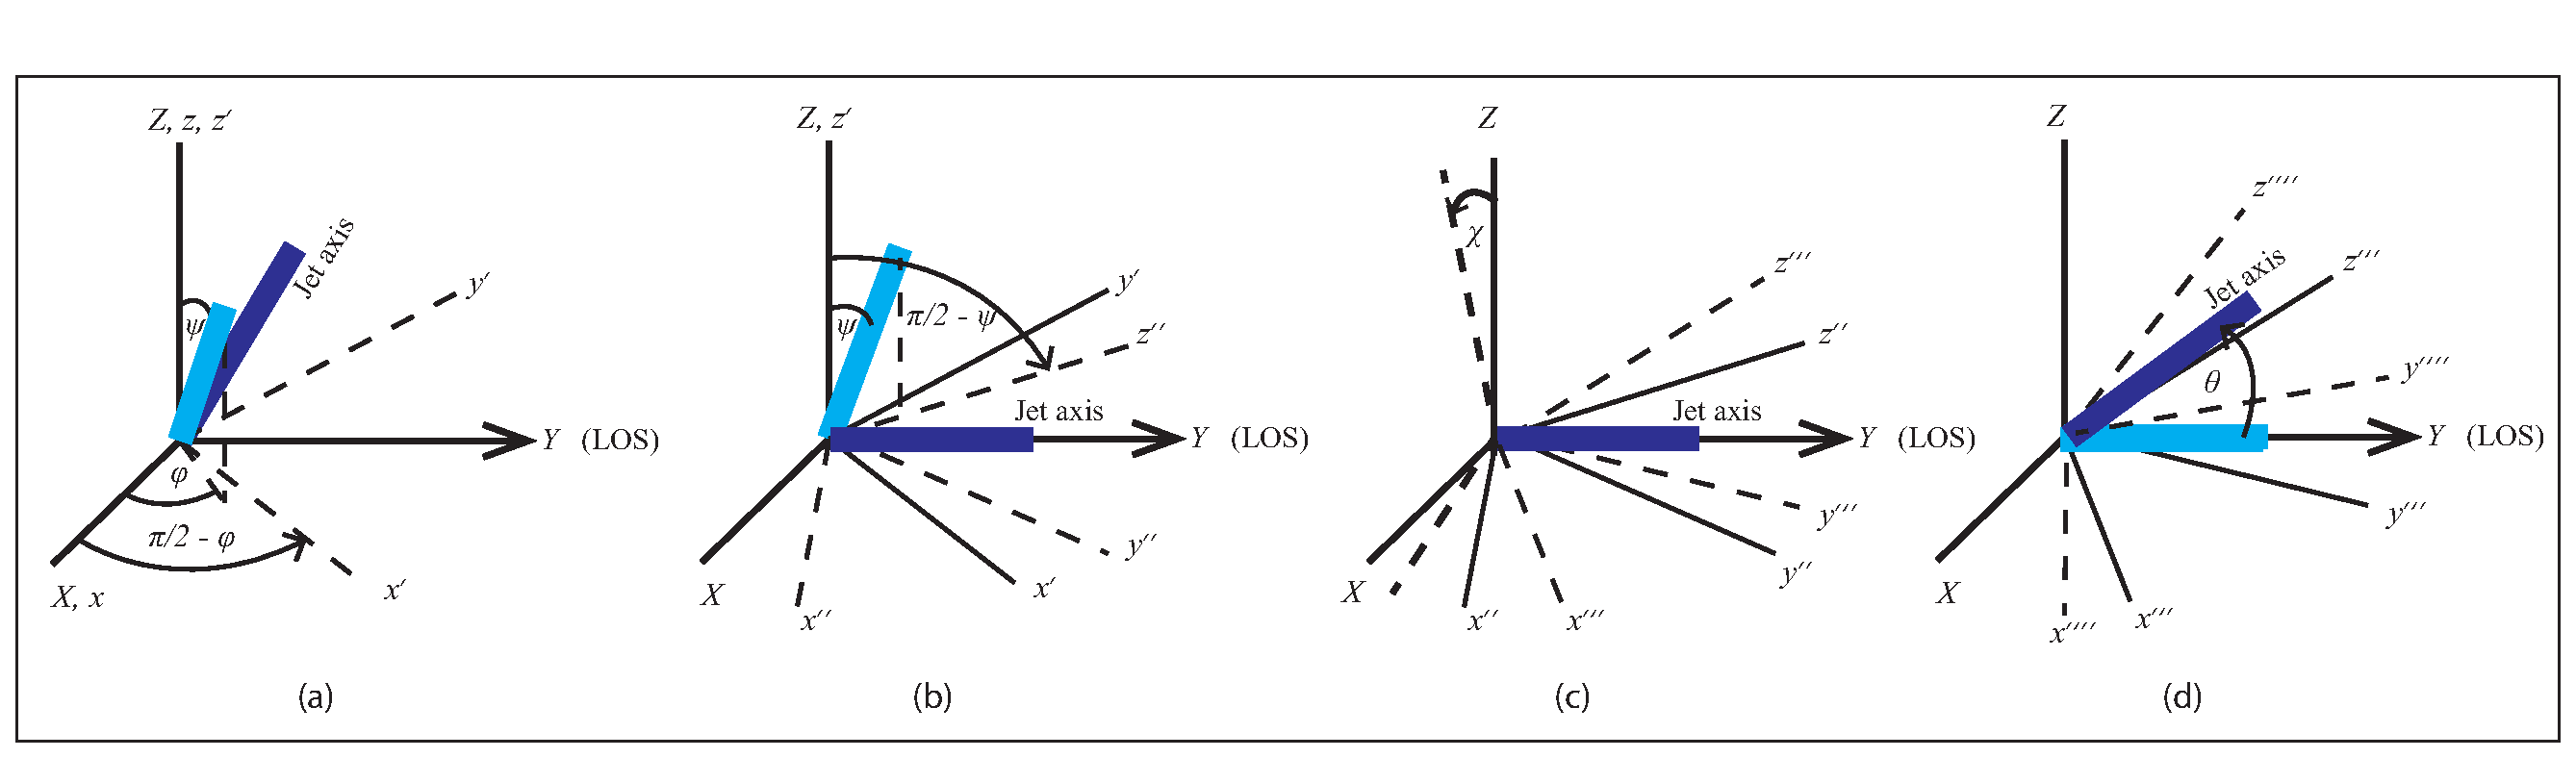
\includegraphics[width=\textwidth]{fig9.eps}
\caption{Transformations of the coordinates associated with the data cube ($xyz$) with respect to coordinates associated with the image cube ($XYZ$) to obtain a line of sight $\theta$ and a viewing direction $\chi$. The line of sight is along the $Y$ axis. See text in Appendix~\ref{A:trans} for details.  }
\label{f:rot}
\end{figure*}
Let $xyz$ be the coordinates (shown in panel (a) of Fig.~\ref{f:rot}) associated with the simulation data cube. At a given time the jet (shown in a blue thick line in panel (a)) makes angles $\psi$ and $\phi$ with the $z$ and $x$ axes. Let $XYZ$ be the coordinates (shown in panel (a) of Fig.~\ref{f:rot}) associated with the synthetic image cube. 
To obtain a desired line of sight and viewing direction we perform the following rotations of the simulation data cube with respect to the synthetic image cube. These rotations are depicted in Fig.~\ref{f:rot}. In each panels of this figure the coordinates associated with the image cubes are shown in bold solid lines, the coordinates associated with the simulation data cubes are in solid (before transformations) and dashed (after transformations) lines, the jets before transformations are in light blue thick lines and the jet after transformations are in dark blue thick lines. 
\begin{enumerate}
\item First we rotate the simulation data cube (anticlockwise) with respect to the $Z$-axis by an angle $\pi/2 - \phi$ (shown in (a)). The coordinates associated with the simulation data cube $xyz$ are transformed to $x'y'z'$. This rotation brings the jet on the $YZ$ plane. The rotation matrix for this rotation $R^{(AC)}_{Z(\pi/2 - \phi)}$ (here the superscript AC denotes the anticlockwise rotation) is given by 
\begin{eqnarray}
R^{(AC)}_{Z(\pi/2 - \phi)}  &=& \begin{pmatrix}
 \cos(\pi/2 - \phi) & -\sin(\pi/2 - \phi) & 0 \\
\sin(\pi/2 - \phi) & \cos(\pi/2 - \phi) & 0 \\
0 & 0 & 1
\end{pmatrix} \nonumber \\
&=& \begin{pmatrix}
 \sin\phi & -\cos\phi & 0 \\
\cos\phi & \sin\phi & 0 \\
0 & 0 & 1
\end{pmatrix} 
\end{eqnarray}
\item We rotate the simulation data cube second time (clockwise) with respect to the $X$-axis by an angle $\pi/2 - \theta$ (shown in panel (b)). The coordinates associated with the simulation data cube $x'y'z'$ are transformed to $x''y''z''$. This rotation makes the jet axis aligned with the line of sight $Y$-axis. The rotation matrix for this rotation $R^{(C)}_{X(\pi/2 - \psi)}$ (the superscript C denotes the clockwise rotation) is given by 
\begin{eqnarray}
R^{(C)}_{X(\pi/2 - \psi)} &=& \begin{pmatrix}
 1 & 0 & 0 \\
0 & \cos(\pi/2 - \psi) & \sin(\pi/2 - \psi) \\
0 & -\sin(\pi/2 - \psi) & \cos(\pi/2 - \psi)
\end{pmatrix} \nonumber \\
& = &\begin{pmatrix}
1 & 0 & 0 \\
0 & \sin\psi & \cos\psi \\
0 & -\cos\psi & \sin\psi
\end{pmatrix}  
\end{eqnarray}
\item Now to obtain a viewing direction we rotate the simulation data cube with respect to the $Y$-axis by an angle $\chi$ (shown in panel (c)). The coordinates associated with the simulation data cube $x''y''z''$ are transformed to $x'''y'''z'''$. The rotation matrix for this rotation $R^{(AC)}_{Y(\chi)} $ is given by
\begin{equation}
R^{(AC)}_{Y(\chi)} = \begin{pmatrix}
 \cos\chi & 0 & \sin\chi \\
0 & 1  & 0 \\
-\sin\chi & 0 & \cos\chi
\end{pmatrix}  
\end{equation}
\item Finally, we rotate the simulation data cube with respect to the $X$-axis by and angle $\theta$ (shown in panel (d)). This rotation relocates the jet (shown in dark blue thick line) at an angle $\theta$ with respect to the $Y$-axis (line of sight). The coordinates associated with the simulation data cube $x'''y'''z'''$ are transformed to $x''''y''''z''''$. The rotation matrix associated with this rotation $R'^{(AC)}_{X(\theta)}$ is given by
 \begin{equation}
  R'^{(AC)}_{X(\theta)} = \begin{pmatrix}
 1 & 0 & 0 \\
0 & \cos\theta & -\sin\theta \\
0 & \sin\theta & \cos\theta 
\end{pmatrix}  
\end{equation}
\end{enumerate} 

The velocity of the fluid in the synthetic image cube $\textbf{v}'$ after the transformations described above is estimated from the velocity in the simulation data cube by using the rotation matrix $R = R'^{(AC)}_{X(\theta)} R^{(AC)}_{Y(\chi)} R^{(C)}_{X(\pi/2 - \psi)} R^{(AC)}_{Z(\pi/2 - \phi)}$
\begin{equation}
\textbf{v}' = R \textbf{v}
\end{equation}

Let $s_1 = \sin \psi$, $s_2 = \sin \phi$, $s_3 = \sin \chi$, $s_4 = \sin \theta$, $c_1 = \cos \psi$,  $c_2 = \cos \phi$, $c_3 = \cos \chi$, and $c_4 = \cos\theta$. Then the rotation matrix $R$ is given by:
 \begin{eqnarray}
  R &=&  R'^{(AC)}_{X(\theta)} R^{(AC)}_{Y(\chi)} R^{(C)}_{X(\pi/2 - \psi)} R^{(AC)}_{Z(\pi/2 - \phi)} \nonumber \\
  &=&  \begin{pmatrix}
  c_3 s_2 - s_3 c_1 c_2  & -c_3 c_2 -s_3 c_1 s_2 & s_3 s_1 \\[6pt]
  c_4 s_1 c_2 + s_4 s_3 s_2  &  c_4 s_1 s_2 + s_4 s_3 c_2 & c_4 c_1 - s_4 c_3 s_1  \\
\phantom{{}+{}}+ s_4 c_3 c_1 c_2 & \phantom{{}+{}}- s_4 c_3 c_1 s_2  & & \\[6pt]
   s_4 s_1 c_2 - c_4 s_3 s_2 & s_4 s_1 s_2 + c_4 s_3 c_2  &  s_4 c_1 + c_4 c_3 s_1 \\
\phantom{{}+{}} - c_4 c_3 c_1c_2   &\phantom{{}+{}}-c_4 c_3 c_1 s_2  & & \\
\end{pmatrix} \nonumber 
\end{eqnarray}

% \begin{eqnarray}
%  R &=&  R'^{(AC)}_{X(\theta)} R^{(AC)}_{Y(\chi)} R^{(C)}_{X(\pi/2 - \psi)} R^{(AC)}_{Z(\pi/2 - \phi)} \nonumber \\
%  &=&  \begin{pmatrix}
%  c\chi s\phi - s\chi c\psi c\phi  & -c\chi c\phi -s\chi c\psi s\phi & s\chi s\psi \\[6pt]
%  c\theta s\psi c\phi + s\theta s\chi s\phi  &  c\theta s\psi s\phi + s\theta s\chi c\phi & c\theta c\psi - s\theta c\chi s\psi  \\
%\phantom{{}+{}+{}}+ s\theta c\chi c\psi c\phi & \phantom{{}+{}+{}}- s\theta c\chi c\psi s\phi  & & \\[6pt]
%   s\theta s\psi c\phi - c\theta s\chi s\phi & s\theta s\psi s\phi + c\theta s\chi c\phi  &  s\theta c\psi + c\theta c\chi s\psi \\
%\phantom{{}+{}+{}} - c\theta c\chi c\psi c\phi   &\phantom{{}+{}+{}}-c\theta c\chi c\psi s\phi  & & \\
%\end{pmatrix} \nonumber 
%\end{eqnarray}

%where $s$ and $c$ stands for $\sin$ and $\cos$ respectively. 

% \cos\chi \sin\phi - \sin\chi \cos\psi \cos\phi  & -\cos\chi \cos\phi -\sin\chi \cos\psi \sin\phi & \sin\chi \sin\psi \\

\section{Synthetic surface brightness of the source at different $\theta$ and $\chi$}\label{A:morph}
\begin{figure*}
\centering
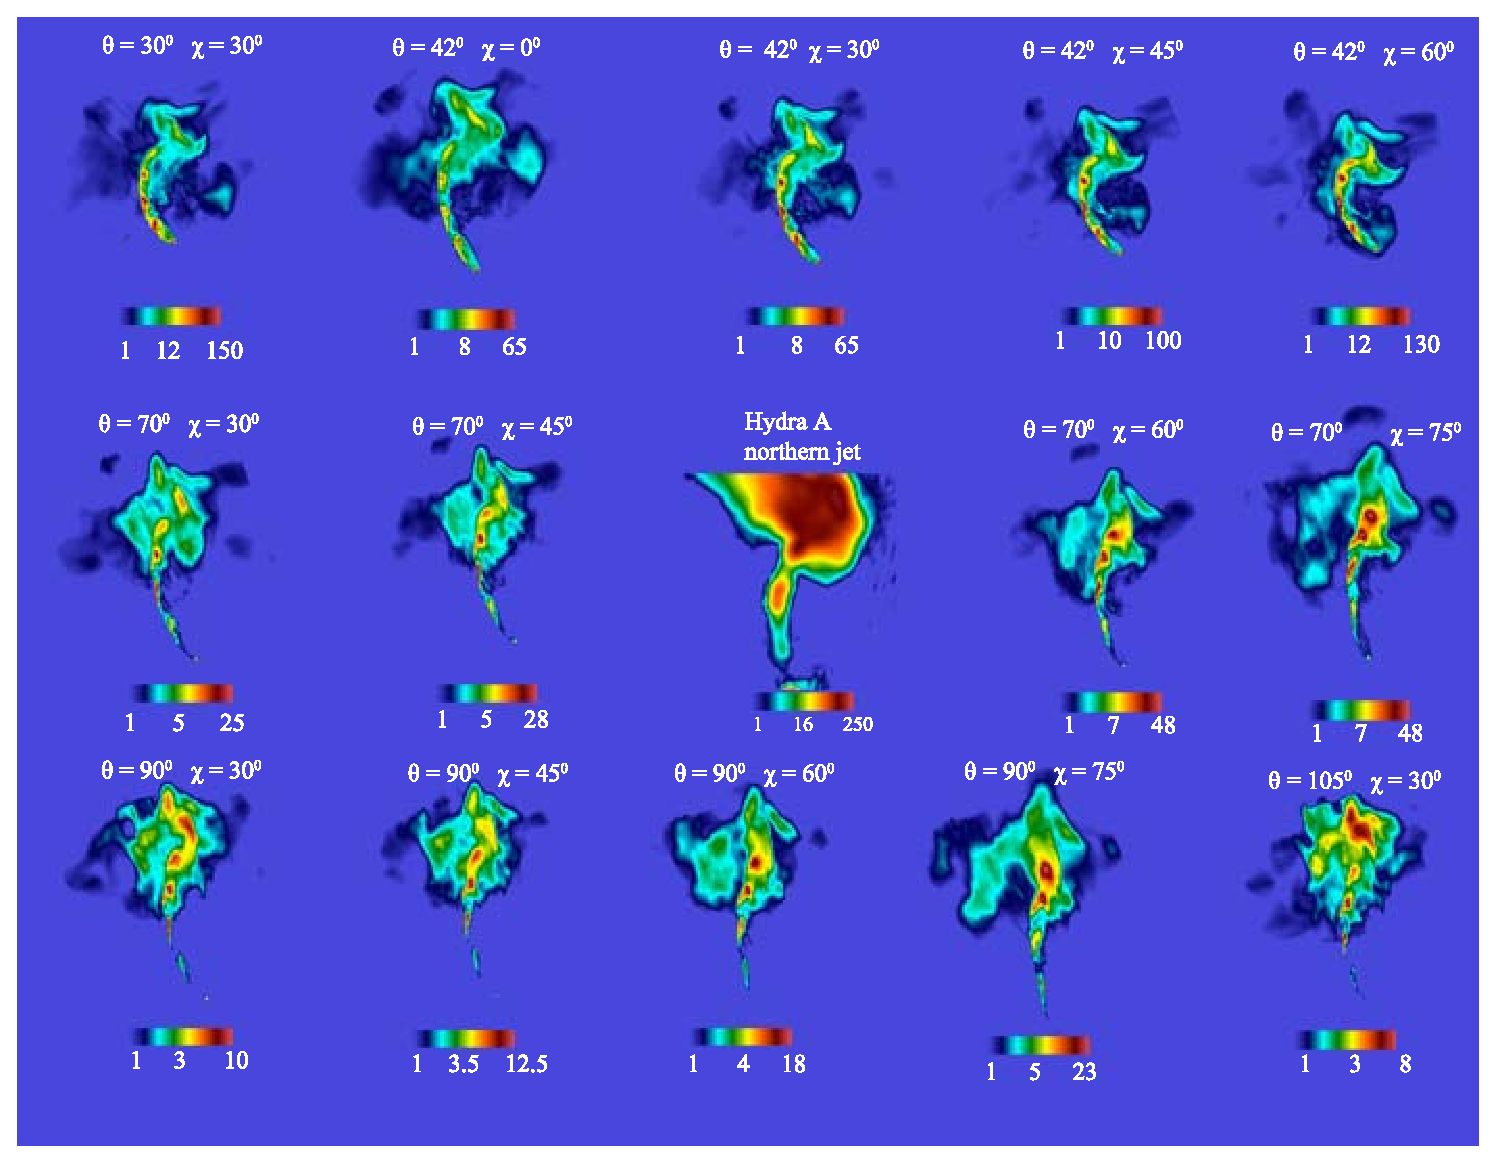
\includegraphics[width=\textwidth]{fig10.eps}
\caption{ Synthetic surface brightness images of the best match model for different line of sights $\theta$ and viewing directions $\chi$. For comparison the observed radio image of the inner 20~kpc of the Hydra A northern jet is shown at the third column of second row. }
\label{f:morph}
\end{figure*}
%
%\section{Jet splitting and misaligned knots at different stages of evolution}\label{A:mknt}
%\begin{figure*}
%\centering
%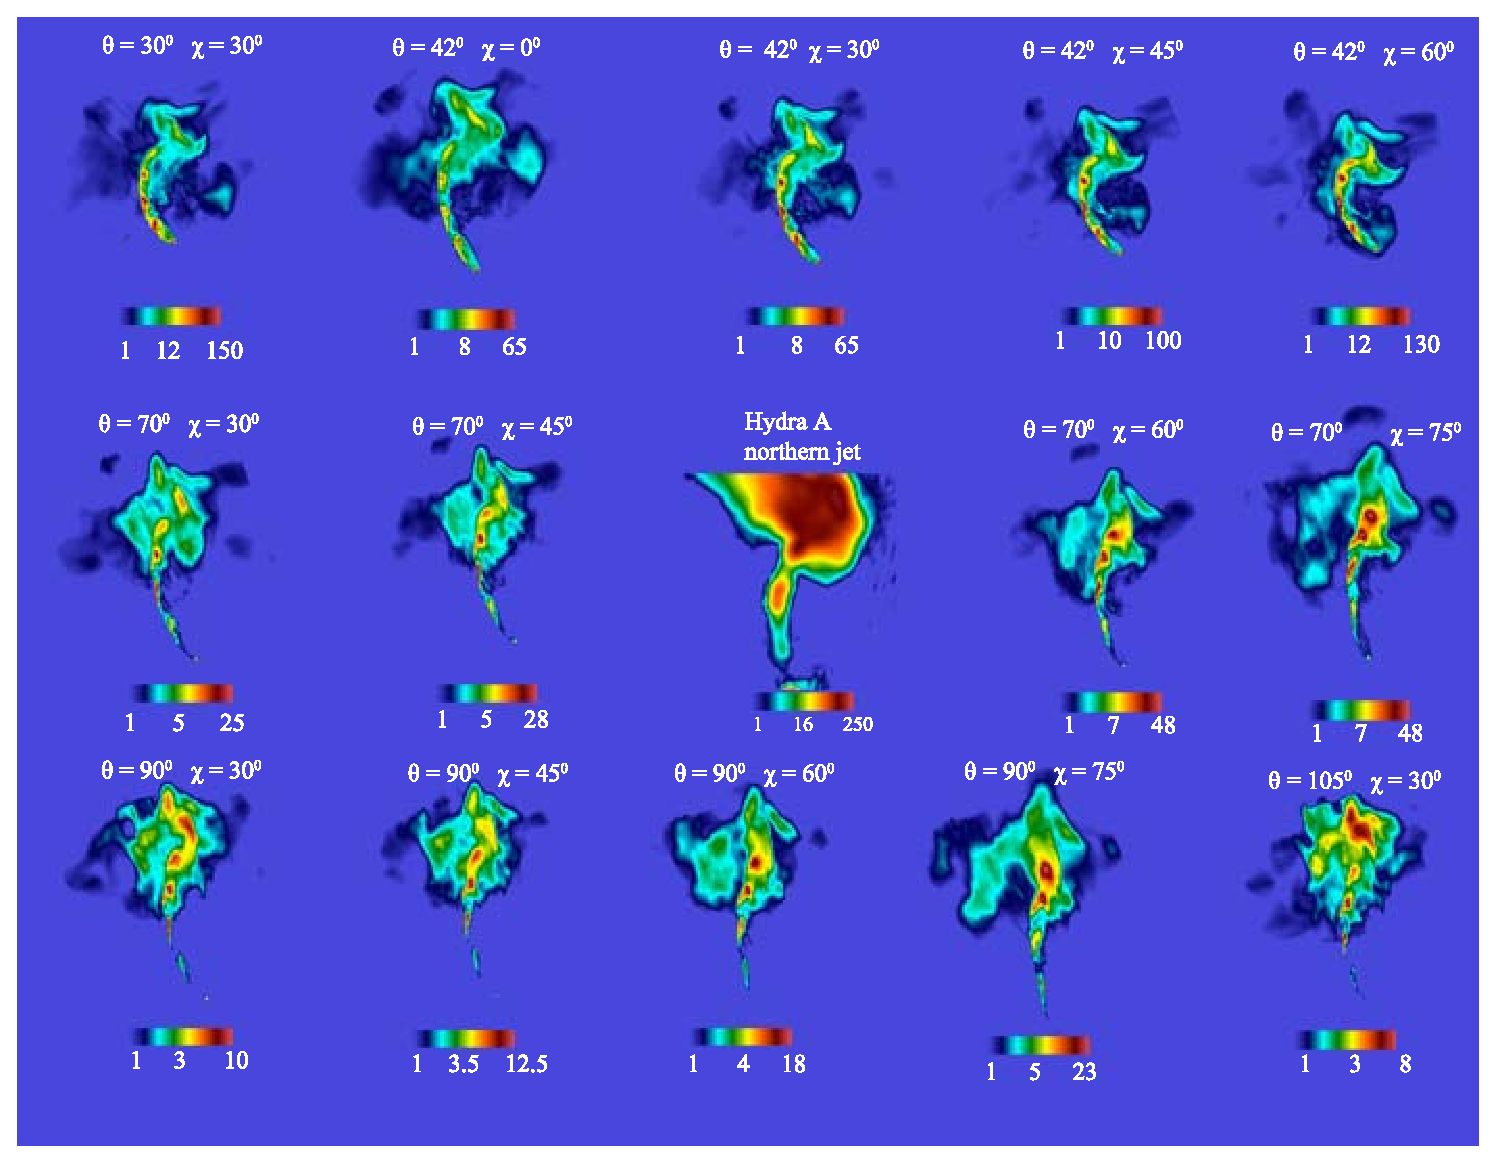
\includegraphics[width=\textwidth]{fig10.eps}
%\caption{ Appearance of jet splitting and misaligned knots at six different stages of evolution of the model A.}
%\label{f:morph}
%\end{figure*}
%
%\bsp
%
%\label{lastpage}
%
\end{document}
